\documentclass[a4paper]{book}
\usepackage[top=2cm, bottom=2cm, left=3cm, right=2cm]{geometry}
\usepackage{amsmath}
\usepackage{graphicx}
\usepackage{hyperref}
\usepackage{amssymb}
\usepackage{amsfonts}
\usepackage{hyperref}
\usepackage[breakable,skins]{tcolorbox}
\usepackage[latin1]{inputenc}
%\usepackage{indentfirst}
\graphicspath{ {./images/} }

\hypersetup{
    colorlinks=true,
    linkcolor=cyan,
    filecolor=magenta,      
    urlcolor=blue,
}

\newtcolorbox{examplebox}[1][]{%
	breakable,
	enhanced,
	colback=yellow!10!white,
	colframe=red,
	coltitle=red,
	#1
}
\newtcolorbox{definitionbox}[1][]{%
	breakable,
	enhanced,
	colback=blue!10!white,
	colframe=blue,
	coltitle=white,
	#1
}
\title{Calculus Single Variable}
\author{Robert Ghrist}
\date{11/15/16}

\begin{document}
\boldmath
\maketitle

\tableofcontents{}

\begin{sloppypar}
\part{Calculus Single Variable}

\chapter{Functions} \label{ChFunctions}

\section{Functions} \label{ChFunctionsSecFunctions}

A \textit{function} can be visualized as a machine that takes in an input $x$ and returns an output $f(x)$. The collection of all possible inputs is called the \textit{domain}, and the collection of all possible outputs is called the \textit{range}.\\
This course deals with functions whose domains and ranges are $\mathbb{R}$ or subsets of $\mathbb{R}$ (this is the notation for the real numbers).\\\\
\textbf{Examples}
\begin{enumerate}
\item Polynomials, e.g. ${f(x) = x^3-5x^2+x+9}$. Give the domain and range of $f$.\\
Answer: The domain is $\mathbb{R}$, because we can plug in any real number into a polynomial. The range is $\mathbb{R}$, which we see by noting that this is a cubic function, so as ${x \rightarrow -\infty}$, ${f(x) \rightarrow -\infty}$, and as ${x \rightarrow \infty}$, ${f(x) \rightarrow \infty}$.
\item Trigonometric functions, e.g. $\sin$, $\cos$, $\tan$. Give the domain and range for each of these.\\
Answer: For $\sin$ and $\cos$: domain is $\mathbb{R}$; range is ${\left[-1,1\right]}$. For $\tan$, the domain is ${\lbrace x \in \mathbb{R}: x \neq \frac{\pi}{2}+k\pi\rbrace}$; range is $\mathbb{R}$.
\item The exponential function, $e^x$. Give the domain and range for the exponential.\\
Answer: Domain is $\mathbb{R}$; range is (${(0,\infty)}$.
\item The natural logarithm function, ${\ln x}$. Recall that this is the inverse of the exponential function. Give the domain and range for ${\ln x}$.\\
Answer: Domain is $(0,\infty)$; range is $\mathbb{R}$. Notice how the domain and range of the exponential relate to the domain and range of the natural logarithm.
\item Is ${\sin^{-1}}$ a function? If so, why? If not, is there a way to make it into a function?
\\Answer: ${\sin^{-1}}$ is not a function, because one input has many outputs. For example, ${\sin^{-1}(0) = 0,\pi,2\pi,\ldots}$. By restricting the range of ${\sin^{-1}}$ to ${\displaystyle\left[-\frac{\pi}{2},\frac{\pi}{2}\right]}$, one gets the function $\arcsin$.
\end{enumerate}

\subsection{Operations on Functions} \label{ChFunctionsSubsOperationsOnFunctions}

\textbf{Composition}\\
The \textit{composition} of two functions, $f$ and $g$, is defined to be the function that takes as its input x and returns as its output $g(x)$ fed into $f$.
\begin{equation*} f\circ g(x)=f(g(x)) \end{equation*}
\\
\textbf{Example:}\\
${\sqrt{1-x^{2}}}$ can be thought of as the composition of two functions, $f$ and $g$. If ${g=1-x^{2}}$, $f$ would be the function that takes an input $g(x)$ and returns its square root.\\\\
\textbf{Example:}\\
Compute the composition ${f \circ f}$, i.e. the composition of $f$ with itself, where ${\displaystyle f(x) = \frac{1}{x+1}}$.\\
Answer:\\
We find that
\begin{align*}
f \circ f(x)&=f(f(x))\\
&=f \left(\frac{1}{x+1}\right)\\
&=\frac{1}{1/\left(x+1\right)+1}\\
&=\frac{x+1}{1+x+1}\\
&=\frac{x+1}{x+2}.
\end{align*}
\\\\
\textbf{Inverse}\\
The \textit{inverse} is the function that undoes $f$. If you plug ${f(x)}$ into ${f^{-1}}$, you will get $x$. Notice that this function works both ways. If you plug ${f^{-1}(x)}$ into $f(x)$, you will get back $x$ again.
\begin{equation*} f^{-1}(f(x))=x \end{equation*} 
\begin{equation*} f(f^{-1}(x))=x \end{equation*}
NOTE: ${f^{-1}}$ denotes the inverse, not the reciprocal. ${f^{-1}(x)\neq\frac{1}{f(x)}}$.\\\\
\textbf{Example:}\\
Let's consider ${f(x)=x^{3}}$. Its inverse is ${f^{-1}(x)=x^{\frac{1}{3}}}$.
\begin{equation*} f^{-1}(f(x))=(x^{3})^{\frac{1}{3}}=x \end{equation*}
\begin{equation*} f(f^{-1}(x))=(x^{\frac{1}{3}})^{3}=x \end{equation*}
Notice that the graphs of $f$ and $f^{-1}$ are always going to be symmetric about the line ${y=x}$. That is the line where the input and the output are the same.

\subsection{Classes of Functions} \label{ChFunctionsSubsClassesOfFunctions}
 
\textbf{Polynomials}\\
A polynomial $P(x)$ is a function of the form 
\begin{equation*} P(x)=c_{0}+c_{1}x+c_{2}x^{2}+\dots+c_{n}x^{n} \end{equation*}
The top power $n$ is called the degree of the polynomial. We can also write a polynomial using a summation notation.
\begin{equation*} P(x)=\sum_{k=0}^{n}c_{k}x^{k} \end{equation*}\\
\textbf{Rational functions}\\
Rational functions are functions of the form ${\displaystyle\frac{P(x)}{Q(x)}}$ where each is a polynomial.\\\\
\textbf{Example:}\\
\begin{equation*} \displaystyle\frac{3x-1}{x^{2}+x-6} \end{equation*} is a rational function. You have to be careful of the denominator. When the denominator takes a value of zero, the function may not be well-defined.\\\\
\textbf{Powers}\\
Power functions are functions of the form ${cx^{n}}$, where $c$ and $n$ are constant real numbers.\\
Other powers besides those of positive integers are useful.\\\\
\textbf{Example:}\\
What is ${x^{0}}$ ?\\
Answer:\\
${x^{0}=1}$\\\\
What is ${x^{-\frac{1}{2}}}$ ?\\
Answer:\\
Recall a fractional power denotes root. For example, ${x^{\frac{1}{2}}=\sqrt{x}}$. The negative sign in the exponent means that we take the reciprocal. So, ${x^{-\frac{1}{2}}=\frac{1}{\sqrt{x}}}$.\\\\
What is ${x^\frac{22}{7}}$ ?\\
Answer:\\
One can rewrite this as ${\left(x^{22}\right)^{1/7}}$. That means we take $x$ to the 22nd power and then take the 7th root of the result.\\
${x^\frac{22}{7}=\sqrt[7]{x^{22}}}$\\\\
What is ${x^{\pi}}$ ? We are not yet equipped to handle this, but we will come back to it later.\\\\
\textbf{Trigonometrics}\\
You should be familiar with the basic trigonometric functions $\sin$, $\cos$. One fact to keep in mind is ${\cos^{2} \theta +\sin^{2} \theta=1}$ for any $\theta$. This is known as a \textit{Pythagorean identity}, which is so named because of one of the ways to prove it:
\begin{center}
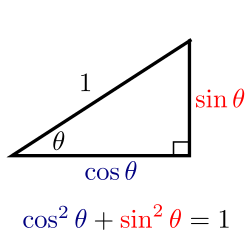
\includegraphics[scale=0.6]{Pythagorean}
\end{center}
By looking at a right triangle with hypotenuse 1 and angle $\theta$, and labeling the adjacent and opposite sides accordingly, one finds by using Pythagoras' Theorem that ${\cos^2 \theta + \sin^2 \theta = 1}$.\\
Another way to think about it is to embed the above triangle into a diagram for the unit circle where we see that ${\cos\theta}$ and ${\sin\theta}$ returns the x and y coordinates, respectively, of a point on the unit circle with angle $\theta$ to the $x$-axis:
\begin{center}
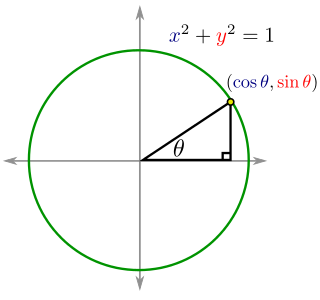
\includegraphics[scale=0.6]{UnitCircle}
\end{center}
That explains the nature of the formula ${\cos^{2} \theta+\sin^{2} \theta=1}$. It comes from the equation of the unit circle ${x^2 + y^2 = 1}$.\\
Others trigonometric functions:\\
${\tan=\displaystyle\frac{\sin}{\cos}}$\\
${\cot=\displaystyle\frac{\cos}{\sin}}$ , the reciprocal of $\tan$\\
${\sec=\displaystyle\frac{1}{\cos}}$ , the reciprocal of the $\cos$\\
${\csc=\displaystyle\frac{1}{\sin}}$ , the reciprocal of the $\sin$\\\\
All four of these have vertical asymptotes at the points where the denominator goes to zero.\\\\
\textbf{Inverse Trigonometrics}\\
We often write ${\sin^{-1}}$ to denote the inverse, but this can cause confusion. Be careful that ${\sin^{-1}\neq\displaystyle\frac{1}{\sin}}$. To avoid the confusion, the terminology $\arcsin$ is recommended for the inverse of the $\sin$ function.\\
The $\arcsin$ function takes on values ${\left[-\displaystyle\frac{\pi}{2},\frac{\pi}{2}\right]}$ and has a restricted domain ${\left[-1,1\right]}$.\\
The $\arccos$ function likewise has a restricted domain ${\left[-1,1\right]}$, but it takes values ${\left[0,\pi\right]}$.\\
The $\arctan$ function has an unbounded domain, it is well defined for all inputs. But it has a restricted range ${\displaystyle\left(-\frac{\pi}{2},\frac{\pi}{2}\right)}$.\\\\
\textbf{Exponentials}\\
Exponential functions are of the form ${c^x}$, where $c$ is some positive constant. The most common such function, referred to as \textit{the} exponential, is ${e^x}$. This is the most common because of its nice integral and differential properties (below).\\
Algebraic properties of the exponential function:\\
\begin{equation*} \displaystyle e^{x}e^{y}=e^{x+y} \end{equation*}
\begin{equation*} \displaystyle (e^{x})^{y}=e^{xy} \end{equation*}
Differential/integral properties:\\
\begin{equation*} \displaystyle\frac{d}{dx} e^{x}=e^{x} \end{equation*}
\begin{equation*} \displaystyle\int e^{x}dx=e^{x}+C \end{equation*}
Recall the graph of ${e^x}$, plotted here alongside its inverse, ${\ln x}$:\\
\begin{center}
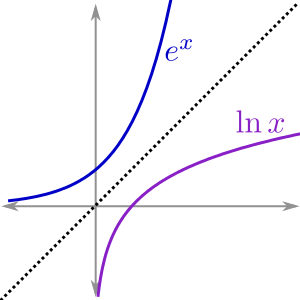
\includegraphics[scale=0.6]{ExpLn}
\end{center}
Note that the graphs are symmetric about the line ${y = x}$ (as is true of the graphs of a function and its inverse).\\
Before continuing, one might ask, what is $e$? There are several ways to define $e$, which will be revealed soon. For now, it is an irrational number which is approximately 2.718281828.\\\\
\textbf{Euler's Formula}\\
To close this lesson, we give a wonderful formula, which for now we will just take as a fact:\\
\begin{examplebox}
Euler's Formula
\begin{equation*} e^{ix}=\cos x+i\sin x \end{equation*}
\end{examplebox}
The $i$ in the exponent is the imaginary number ${\sqrt{-1}}$. It has the properties ${i^{2}=-1}$. $i$ is not a real number. That doesn't mean that it doesn't exist. It just means it is not on a real number line.\\
Euler's formula concerns the exponentiation of an imaginary variable. What exactly does that mean? How is this related to trigonometric functions? This will be covered in our next lesson.\\\\
\textbf{Additional Examples}\\\\
\textbf{Example:}\\
Find the domain of \[ f(x) = \frac{1}{\sqrt{x^2 -3x+2}}. \]
Answer:\\
te that the square root is only defined when its input is non-negative. Also, the denominator in a rational function cannot be 0. So we find that this function is well-defined if and only if ${x^2-3x+2>0}$. Factoring gives \[ (x-2)(x-1) > 0. \]
By plotting the points ${x=1}$ and ${x=2}$ (where the denominator equals 0) and testing points between them, one finds that ${x^2-3x+2>0}$ when ${x<1}$ or ${x>2}$:
\begin{center}
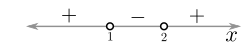
\includegraphics[scale=0.6]{PointChecking}
\end{center}
So the domain of $f$ is ${x<1}$ or ${2<x}$. In interval notation, this is ${\left(-\infty,1\right) \cup \left(2, \infty \right)}$.\\\\
\textbf{Example:}\\
Find the domain of \[ f(x) = \ln(x^3-6x^2+8x). \]
Answer:\\
Since $\ln$ is only defined on the positive real numbers, we must have ${x^3-6x^2+8x>0}$. Factoring gives \[ x(x^2-6x+8) = x(x-2)(x-4)>0 \]
As in the above example, plotting the points where this equals 0 and then testing points, we find that the domain is ${0<x<2}$ and ${4<x}$. In interval notation, this is ${\left(0,2 \right) \cup \left(4,\infty\right)}$.

\section{The Exponential} \label{ChFunctionsSecTheExponential}

This module deals with a very important function: the exponential. The first question one might ask is: what is the exponential function ${e^x}$? We know certain values of the function such as ${e^0=1}$, but what about an irrational input such as ${e^\pi}$, or an imaginary input ${e^i}$? Is it possible to make sense of these values?\\
The following definition answers these questions.\\
\begin{examplebox}
The Exponential $e^x$
\begin{align*} 
e^x &= 1+x+\frac{x^2}{2!} + \frac{x^3}{3!} + \frac{x^4}{4!} + \dotsb 
& = \sum_{k=0}^\infty \frac{x^k}{k!}, 
\end{align*}
where \[ k! = k(k-1)(k-2)\dotsb 3 \cdot 2 \cdot 1, \] and ${0! = 1}$
\end{examplebox}
One can now plug values for $x$ into the above sum to compute ${e^x}$. When ${x=0}$, for instance, one finds that ${e^0=1}$, (since all the terms with $x$ disappear) as expected. By plugging in ${x=1}$, the true value of $e$ is found to be ${e=1+1+\frac{1}{2!}+\frac{1}{3!}+\dotsb}$.\\\\

\subsection{A long polynomial}

There are technical concerns when trying to add up an infinite number of things. These issues will be dealt with later in the modules on \hyperref[ChDiscretizationSecSeries]{series}. For now, treat the infinite sum above as a long polynomial (the actual term is the Taylor series about ${x=0}$, which will be more formally dealt with in the \hyperref[ChFunctionsSecTaylorSeries]{next module}). Polynomials are nice because they are easy to integrate and differentiate. Recall the power rule for differentiating and integrating a monomial ${x^k}$, where $k$ is a constant:
\begin{align*}
\frac{d}{dx} x^k &= kx^{k-1} 
\int x^k \, dx &= \frac{1}{k+1} x^{k+1} + C \quad (k \neq -1) 
\end{align*}

\subsection{Properties of $e^x$}

Recall the following properties of the exponential function:
\begin{enumerate}
\item ${e^{x+y} = e^xe^y}$
\item ${e^{x\cdot y}=(e^x)^y=(e^y)^x}$
\item ${\frac{d}{dx}e^x = e^x}$
\item ${\int e^x dx=e^x+C}$.
\end{enumerate}
Consider the last two properties in terms of the long polynomial.Taking the derivative of the long polynomial for ${e^x}$ gives
\begin{align*} 
\frac{d}{dx}(1+x+\frac{x^2}{2!}+\frac{x^3}{3!} + \frac{x^4}{4!} + \dotsb)
&= 0 + 1 + \frac{2x}{2!} + \frac{3x^2}{3!} + \frac{4 x^3}{4!} + \dotsb\\
&= 1 + x + \frac{x^2}{2!} + \frac{x^3}{3!} + \dotsb,
\end{align*}
which is the original long polynomial. Integrating also gives (up to the constant of integration) the original long polynomial. This agrees with facts about the derivative and integral of ${e^x}$. Thus, the long polynomial for ${e^x}$ captures two of the key features of ${e^x}$; namely, ${e^x}$ is its own derivative and its own integral.

\subsection{Euler's formula}

Recall that the imaginary number $i$ is defined by ${i=\sqrt{-1}}$. So ${i^2=-1}$, ${i^3=-i}$, ${i^4=1}$, and this continues cyclically (for a review of complex/imaginary numbers, see \href{https://en.wikipedia.org/wiki/Complex_number}{wikipedia}). Assume the following fact, known as Euler's formula, mentioned in the last module.
\begin{examplebox}
	Euler's formula
	\begin{equation*} e^{ix} = \cos x + i \sin x. \end{equation*}
\end{examplebox}
Consider what happens when $ix$ is plugged into the long polynomial for ${e^x}$. By simplifying the powers of $i$, and grouping the result into its real and imaginary parts, one finds
\begin{align*} 
e^{ix} &= 1+ix+\frac{(ix)^2}{2!}+\frac{(ix)^3}{3!} + \dotsb\\
&= 1 + ix + \frac{i^2 x^2}{2!} + \frac{i^3 x^3}{3!} + \dotsb\\
&= 1 + ix - \frac{x^2}{2!} - i\frac{x^3}{3!} + \frac{x^4}{4!} + i \frac{x^5}{5!} + \dotsb\\
&= \left(1 - \frac{x^2}{2!} + \frac{x^4}{4!} - \dotsb\right) + i \left(x - \frac{x^3}{3!} + \frac{x^5}{5!} - \dotsb \right).
\end{align*}
If this is supposed to equal ${\cos x + i \sin x}$, then the real part must be ${\cos x}$, and the imaginary part must be ${\sin x}$. It follows that
\begin{align*}
\cos x &= 1 - \frac{x^2}{2!} + \frac{x^4}{4!} - \frac{x^6}{6!} + \dotsb = \sum_{k=0}^\infty (-1)^k \frac{x^{2k}}{(2k)!} \\
\sin x &= x - \frac{x^3}{3!} + \frac{x^5}{5!} - \frac{x^7}{7!} + \dotsb = \sum_{k=0}^\infty (-1)^k \frac{x^{2k+1}}{(2k+1)!}.
\end{align*}
These formulas should be memorized, both in their long polynomial form and their more concise summation notation form.\\\\
\textbf{Example:}\\
Compute ${1-\frac{\pi^2}{2!}+\frac{\pi^4}{4!}-\dotsb}$.\\
Answer:\\
Note that this is the long polynomial for ${\cos x}$, evaluated at ${x=\pi}$. So the value is ${\cos \pi = -1}$.\\\\
\textbf{Example:}\\
Check that taking the derivative of the long polynomial for ${\sin x}$ gives the long polynomial for ${\cos x}$ (hence, verify that ${\frac{d}{dx} \sin x = \cos x}$.\\
Answer:\\
Computing the derivative term by term gives
\begin{align*}
\frac{d}{dx} \sin(x) &= \frac{d}{dx} \left(x - \frac{x^3}{3!} + \frac{x^5}{5!} - \ldots \right) \\
&= 1 - 3 \frac{x^2}{3!} + 5 \frac{x^4}{5!} - \ldots \\
&= 1 - \frac{x^2}{2!} + \frac{x^4}{4!} - \ldots,
\end{align*}
which is the long polynomial for ${\cos x}$, as desired.\\\\
\textbf{Example:}\\
Show that the long polynomial for ${e^x}$ satisfies the first property above, namely ${e^{x+y} = e^x e^y}$. Hint: start with the long polynomials for ${e^x}$ and ${e^y}$ and multiply these together, and carefully collect like terms to show it equals the long polynomial for ${e^{x+y}}$.\\
Answer:\\
Beginning with ${e^x \cdot e^y}$, we find
\begin{align*}
e^x \cdot e^y &= \left(1+ x + \frac{x^2}{2!} + \dotsb \right) \left(1 + y + \frac{y^2}{2!} + \dotsb \right) \\
&= 1 + (x+y) + \left( \frac{x^2}{2!} + xy + \frac{y^2}{2!} \right) + \dotsb \\
&= 1 + (x+y) + \frac{x^2 + 2xy + y^2}{2!} + \dotsb \\
&= 1 + (x+y) + \frac{(x+y)^2}{2!} + \dotsb,
\end{align*}
which is the long polynomial for ${e^{x+y}}$, as desired.

\subsection{More on the long polynomial}

The idea of a long polynomial is reasonable, because it actually comes from taking a sequence of polynomials with higher and higher degree:
\begin{align*} 
f_0(x) &= 1 \\
f_1(x) &= 1+x \\
f_2(x) &= 1+x+\frac{x^2}{2} \\
f_3(x) &= 1+ x+ \frac{x^2}{2} + \frac{x^3}{6} \\
&\vdots. 
\end{align*}
Each polynomial in the sequence is, in a sense, the best approximation possible of that degree. Put another way, taking the first several terms of the long polynomial gives a good polynomial approximation of the function. The more terms included, the better the approximation. This is how calculators compute the exponential function (without having to add up infinitely many things).
\begin{center}
	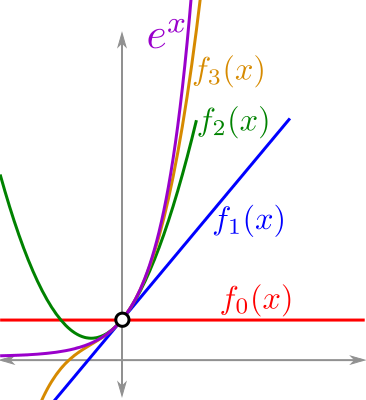
\includegraphics[scale=0.6]{ExponentialApproximants}
\end{center}
\noindent\makebox[\linewidth]{\rule{\paperwidth}{0.4pt}}

\subsection{Exercises}
\begin{itemize}
	\item So, how good of an approximation is a polynomial truncation of ${e^x}$? Use a calculator to compare how close $e$ is to the linear, quadratic, cubic, quartic, and quintic approximations. How many digits of accuracy do you seem to be gaining with each additional term in the series?
	\item Now, do the same thing with ${1/e}$ by plugging in ${x=-1}$ into the series. Do you have the same results? Are you surprised?
	\item Use the first three terms of the series for ${e^x}$ to approximate ${\sqrt[10]{e}}$ and ${e^{10}}$. How accurate do you think these approximations are?
	\item Calculate the following sum using what you know: \[\sum_{n=0}^\infty (-1)^n\frac{(\ln 3)^n}{n!}\]
	\item Write out the first four terms of the following series \[\sum_{n=0}^\infty (-1)^n\frac{\pi^{2n}}{2^n n!}\]
	\item Write out the following series using summation notation:\[1-\frac{2}{3!}+\frac{4}{5!}-\frac{8}{7!}+\cdots\]
	\item Estimate ${\sin(1/2)}$ to three digits of accuracy. How many terms in the series did this take?
	\item We've seen that ${i=e^{i\pi/2}}$ via Euler's formula. Using this and some algebra, tell me what is ${i^i}$. Isn't that nice? Now, tell me, what is ($(i^i)^i$)? Are you surprised? That's like, unreal!
	\item Practice your summation notation by rewriting the sum \[\sum_{n=2}^\infty (-1)^n\frac{x^{n-2}}{n^3}\] as a sum over an index that goes from zero to infinity.
	\item Use the first two nonzero terms of the Taylor series for ${\cos(x)}$ to approximate ${\cos(\frac{1}{10})}$.
	\item Use Euler's formula to derive the double angle formulas ${\cos(2\theta)=\cos^2(\theta)-\sin^2(\theta)}$ and ${\sin(2\theta)=2\sin(\theta)\cos(\theta)}$.
\end{itemize}

\section{Taylor series} \label{ChFunctionsSecTaylorSeries}
The long polynomial from the last module is actually called a Taylor series about ${x=0}$ (this is referred to as a Maclaurin series in some textbooks, but this course will use the term Taylor series). The last module gave the Taylor series for ${e^x}$, ${\sin x}$, and ${\cos x}$. The logical next question is to ask whether every function has a Taylor series.\\
The answer is that most \textit{reasonable} functions, and almost all of the functions encountered in this course, have a Taylor series. That is, every reasonable function $f$ can be written as \[f(x)=\sum_{k=0}^\infty c_k x^k=c_0+c_1 x+c_2 x^2+\dotsb.\]
This module describes how to compute the coefficients $c_k$ for a given function $f$.

\subsection{The definition of a Taylor series at x=0}
The definition of the Taylor series of $f$ at ${x=0}$ is
\begin{examplebox}
	Taylor series at ${x=0}$
	\begin{equation*}	
	f(x) = f(0) + \frac{f'(0)}{1!}x + \frac{f(0)}{2!}x^2 + \frac{f'(0)}{3!}x^3+\dotsb = \sum_{k=0}^\infty \frac{f^{\left(k\right)}(0)}{k!} x^k,
	\end{equation*}
	where ${f^{\left(k\right)}(0)}$ is the $k$th derivative of $f$ evaluated at 0. In other words, the coefficient $c_k$ mentioned above is given by \[c_k=\frac{f^{\left(k\right)}(0)}{k!}=\frac{1}{k!}\cdot\frac{d^k f}{dx^k}\bigg|_0\] 
\end{examplebox}
This seems circular, since the definition uses the function, and its derivatives, to write down the function. However, the definition only actually requires information about the function at a single point (in this case, 0). It is best to think of the Taylor series as a way of turning a function into a polynomial.\\
\textbf{Example} Compute the Taylor series for $e^x$ using the above definition to see that it matches the given series from the last module.\\
Answer:\\
Here, ${f(x)=e^x}$, and every derivative of $e^x$ is $e^x$. Therefore, for all $k$ we have \[f^{\left(k\right)}(x)=e^x,\] and so ${f^{\left(k\right)}(0)=1}$ for all $k$. Plugging into the Taylor series formula gives
\begin{align*}
f(x) &= \sum_{k=0}^\infty \frac{f^{\left(k\right)}(0)}{k!} x^k \\
&= \sum_{k=0}^\infty \frac{x^k}{k!} \\
&= 1 + x + \frac{x^2}{2!} + \frac{x^3}{3!} + \dotsb, 
\end{align*}
as claimed.\\\\
\textbf{Example} Compute the Taylor series for ${f(x)=\sin x}$ using the above definition, and verify it matches the series found using Euler's formula.\\
Answer:\\
Computing the derivatives, and then evaluating at ${x=0}$ gives the following table:
\begin{align*}
f(x) &= \sin(x) & f(0) &= 0 \\
f'(x) &= \cos(x) & f'(0) &= 1 \\
f''(x) &= -\sin(x) & f''(0) &= 0 \\
f'''(x) &= -\cos(x) & f'''(0) &= -1 \\
& \vdots 
\end{align*}
Thus,
\begin{align*}
\sin(x) &= 0+\frac{1}{1!}x+\frac{0}{2!}x^2+\frac{-1}{3!}x^3+\dotsb \\
&= x - \frac{x^3}{3!} + \frac{x^5}{5!} - \dotsb,
\end{align*}
confirming what was found last time.\\\\
\textbf{Example} Compute the Taylor series for ${f(x) = x^2-5x+3}$.\\
Again, by directly using the definition:
\begin{align*}
f(x) &= x^2-5x+3 & f(0) &= 3 \\
f'(x) &= 2x-5 & f'(0) &= -5 \\
f''(x) &= 2 & f''(0) &= 2 \\
f'''(x) &= 0 & f'''(0) &= 0 \\
& \vdots
\end{align*}
So it follows that \[f(x)=3-5x+\frac{2}{2!}x^2=3-5x+x^2\]
(since all the subsequent derivatives are 0), which is the original function. This should not be a surprise, since the Taylor series represents a function as a long polynomial (henceforth called by its proper name: \textit{series}). If $f$ was a polynomial to begin with, it stands to reason that the Taylor series for $f$ should just be $f$ itself.

\subsection{Why Taylor series matter}
The big idea of this module is that the Taylor series can be thought of as an operator (a machine) which turns a function into a series. This is a useful operator because some functions are hard (or even impossible) to express using combinations of familiar functions. Nevertheless, these functions can often be understood by computing their Taylor series.\\
\textbf{Example} The \textit{Bessel function}, denoted $J_0$, is best defined by its Taylor series:
\begin{align*} 
J_0 &= \sum_{k=0}^\infty (-1)^k \frac{x^{2k}}{2^{2k} (k!)^2} \\
&= 1 - \frac{1}{2^2} x^2 + \frac{1}{2^4(2!)^2}x^4 - \frac{1}{2^6 (3!)^2}x^6 + \dotsb 
\end{align*}
This series has only the even powers of $x$, and it alternates, which is reminiscent of the series for cosine. One difference is that the denominator in the Bessel function grows more quickly than the denominator in the series for cosine. Thus, we might expect the graph to be a wave with a decreasing amplitude, which is exactly what we find:
\begin{center}
	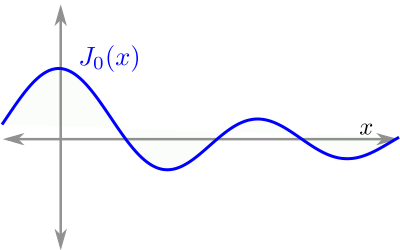
\includegraphics[scale=0.6]{Bessel}
\end{center}
It turns out that the Bessel function describes many physical phenomena, including the shape of a hanging chain as it is rotated, and the shape of the waves formed after a stone is thrown into a pool of water.

\subsection{Taylor series as polynomial approximants}
The main reason Taylor series are useful is that they turn a potentially complicated function into something simple: a polynomial. Granted, this polynomial is infinitely long in general, but in practice it is only necessary to compute the first few terms to get a good, local approximation of the function. The more terms one includes, the better the polynomial approximates the function.\\
As an example, consider a particle on the number line with position function $p(t)$. At time 0, say its position is 5. Then one approximation of its position as a function of time is ${p_0(t)=5}$. Given more information, say its velocity at time 0 is 3, the approximation becomes better. The next approximation as a function of time is ${p_1(t)=5+3t}$. Now, suppose its acceleration at time 0 is $-4$. Then ${p_2(t)=5+3t-\frac{4}{2}t^2=5+3t-2t^2}$ is an even better polynomial approximation of the position function.\\
\begin{center}
	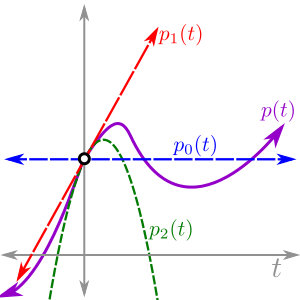
\includegraphics[scale=0.6]{Approximants}
\end{center}
\noindent\makebox[\linewidth]{\rule{\paperwidth}{0.4pt}}

\subsection{Exercises}
\begin{itemize}
\item What is the Taylor series of ${x^4-3x^3+2x^2+7x-3}$. This should be an easy one!
\item What is the Taylor series of ${(x-2)^2(x-3)}$? This, also, should not be *too* hard...
\item Compute a few derivatives and figure out the first few terms of the Taylor series of ${\displaystyle\frac{1}{1-x}}$. Have you seen this series before?
\item What are the first two nonzero terms in the Taylor series of ${\sqrt[3]{1-2x}}$?
\item What is the coefficient of the cubic term in the Taylor series of ${e^{-3x}}$?
\item Use what you know about Taylor series to determine the third derivative of ${\sin^3(2x)\cos^2(3x)}$ at ${x=0}$. That's a *lot* easier than computing the derivatives!
\item The ERF function is defined in terms of a difficult integral: \[ERF(x)=\frac{2}{\sqrt{\pi}}\int_0^x e^{-t^2}\,dt\]
\item Even if you don't remember integrals all that well, you know how to integrate a polynomial, right? So, Taylor expand the integrand and integrate term by term to get the Taylor series for ERF.
\item What is the third derivative of ERF(x) at zero?
\item Why does a Taylor series have all those ($n!$) terms in the denominator? Let's see. Compute the Taylor series of ${f(x)=(1+x)^5}$ by (1) using the binomial theorem (or multiplication) to expand that power; then (2) by differentiating the function and using the Taylor series formula. What do you notice when you keep computing higher derivatives?
\end{itemize}

\section{Computing Taylor series} \label{ChFunctionsSecComputingTaylorSeries}
The previous module gave the definition of the Taylor series for an arbitrary function. It turns out that this is not always the easiest way to compute a function's Taylor series. Just as functions can be added, subtracted, multiplied, and composed, so can their corresponding Taylor series.\\
Recall that the Taylor series for a function ($f$) is given by \[f(x)=\sum_{k=0}^\infty \frac{f^{\left(k\right)}(0)}{k!} x^k=f(0)+f'(0)x+\frac{f''(0)}{2!} x^2+\dotsb.\]
Using the definition of the Taylor series involves taking a lot of derivatives, which could be a lot of work, especially if the function involves compositions and products of functions, e.g. ${f(x)=\sin(x^2)e^{x^3}}$. This module will show how to compute the Taylor series of such functions more easily by using the Taylor series for functions we already know.

\subsection{Substitution}
Our first method, substitution, allows us to plug one function into the Taylor series of another. Consider the function \[f(x)=\frac{1}{x}\sin(x^2).\]
Computing the Taylor series for $f$ from the definition would involve the quotient rule, chain rule, and a lot of algebra. But by taking the series for ${\sin x}$ and substituting $x^2$ into this series, and then distributing the ${\frac{1}{x}}$, one finds
\begin{align*}
\frac{1}{x}\sin(x^2)&=\frac{1}{x}\left((x^2)-\frac{1}{3!}(x^2)^3+\frac{1}{5!}(x^2)^5-\dotsb\right) \\
&=\frac{1}{x}\left(x^2-\frac{1}{3!}x^6+\frac{1}{5!}x^{10}-\dotsb\right) \\
&=x-\frac{1}{3!}x^5+\frac{1}{5!}x^9-\dotsb. 
\end{align*}
Note that getting this many terms using the definition would involve taking nine derivatives of the original function, which would be a lot of work! To get a more complete description of the Taylor series, one can use the summation notation, and again substitute to find
\begin{align*}
\frac{1}{x} \sin(x^2) &= \frac{1}{x} \sum_{k=0}^\infty (-1)^k \frac{(x^2)^{2k+1}}{(2k+1)!} \\
&= \frac{1}{x} \sum_{k=0}^\infty (-1)^k \frac{x^{4k+2}}{(2k+1)!} \\
&= \sum_{k=0}^\infty (-1)^k \frac{x^{4k+1}}{(2k+1)!}
\end{align*}
\textbf{Example} Find the Taylor series for ${e^{x^3}}$ by substitution.\\
Answer:\\
Recall the series for $e^x$ is \[e^x=1+x+\frac{x^2}{2!}+\frac{x^3}{3!}+\dotsb=\sum_{k=0}^\infty\frac{x^k}{k!}\]
Substituting $x^3$ into the series for $e^x$ gives
\begin{align*}
e^{x^3} &= 1 + x^3 + \frac{(x^3)^2}{2!} + \frac{(x^3)^3}{3!} + \dotsb \\
&= 1 + x^3 + \frac{x^6}{2!} + \frac{x^9}{3!} + \dotsb \\
&= \sum_{k=0}^\infty \frac{(x^3)^k}{k!} \\
&= \sum_{k=0}^\infty \frac{x^{3k}}{k!}
\end{align*}

\subsection{Combining like terms}
Another way to use previous knowledge of one Taylor series to find another is by combining like terms. This requires some careful algebra, but it is no more difficult than multiplying two polynomials together. For example, consider the function \[f(x)=\cos^2(x)=\cos(x)\cdot\cos(x).\]
Finding the series for a function multiplied by another function is the same as taking the series for each function and multiplying them together, and then collecting like terms. This is where some algebra is required.
\begin{align*}
\cos(x)\cdot\cos(x)&=\left(1-\frac{1}{2!}x^2+\frac{1}{4!}x^4-\dotsb\right)\left(1-\frac{1}{2!}x^2+\frac{1}{4!}x^4-\dotsb\right) \\ 
&=1+\left(-\frac{1}{2!}-\frac{1}{2!}\right)x^2+\left(\frac{1}{4!}+\frac{1}{2!}\frac{1}{2!}+\frac{1}{4!}\right)x^4+\dotsb \\
&=1-x^2+\frac{1}{3}x^4+\dotsb.
\end{align*}
To see where the coefficient of $x^4$ comes from, note that every $x^4$ term comes from some term from the left series multiplied together with some term from the right series whose powers add up to 4. There are three such pairs: 1 on the left paired with ${\frac{1}{4!}x^4}$ on the right; ${-\frac{1}{2!}x^2}$ on the left paired with ${-\frac{1}{2!}x^2}$ on the right; and ${\frac{1}{4!}x^4}$ on the left paired with 1 on the right. This is the same algebra one would do when multiplying two polynomials together; this is just a way of collecting like terms in a systematic way.\\\\
\textbf{Example} Use the trigonometric identity \[\cos^2x=\frac{1+\cos(2x)}{2}\] and substitution to find the series for ${\cos^2x}$. Try to give the series in summation notation (other than the first term)\\
Answer:\\
By the above identity,
\begin{align*}
\cos^2x &= \frac{1}{2} \left(1 + \cos(2x)\right) \\
&= \frac{1}{2} \left(1 + \left(1 - \frac{(2x)^2}{2!} + \frac{(2x)^4}{4!} - \dotsb \right)\right) \\
&= \frac{1}{2} \left(2 - \frac{4x^2}{2} + \frac{16x^4}{24} - \dotsb \right) \\
&= 1 - x^2 + \frac{x^4}{3} - \dotsb.
\end{align*}
In summation notation,
\begin{align*}
\cos^2x &= \frac{1}{2} \left(1 + \sum_{k=0}^\infty (-1)^k \frac{(2x)^{2k}}{(2k)!}\right)  \\
&= \frac{1}{2} + \frac{1}{2} \sum_{k=0}^\infty (-1)^k \frac{(2x)^{2k}}{(2k)!} \\
&= \frac{1}{2} + \sum_{k=0}^\infty (-1)^k \frac{2^{2k-1}x^{2k}}{(2k)!} \\
&= 1 + \sum_{k=1}^\infty (-1)^k \frac{2^{2k-1}x^{2k}}{(2k)!}.
\end{align*}

\subsection{Hyperbolic trigonometric functions}
The hyperbolic trigonometric functions ${\sinh(x)}$, ${\cosh(x)}$, and ${\tanh(x)}$ are defined by
\begin{align*}
\sinh(x) &= \frac{e^x - e^{-x}}{2} \\
\cosh(x) &= \frac{e^x+e^{-x}}{2} \\
\tanh(x) &= \frac{e^x - e^{-x}}{e^x + e^{-x}} = \frac{\sinh(x)}{\cosh(x)}.
\end{align*}
\begin{center}
	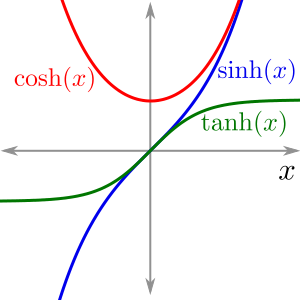
\includegraphics[scale=0.6]{Hyperbolic}
\end{center}
These hyperbolic trig functions, although graphically quite different from their traditional counterparts, have several similar algebraic properties, which is why they are so named. For example, the Pythagorean identity for cosine and sine has a version for hyperbolic cosine and sine: \[\cosh^2(x)-\sinh^2(x)=1.\]
One can verify this using the definitions and some algebra. But there is a geometric intuition for this relationship. Recall that cosine and sine give the $x$ and $y$ coordinates, respectively, for a point on the unit circle ${x^2+y^2=1}$. The hyperbolic cosine and hyperbolic sine give the $x$ and ($y$) coordinates, respectively, for points on the hyperbola ${x^2-y^2=1}$:
\begin{center}
	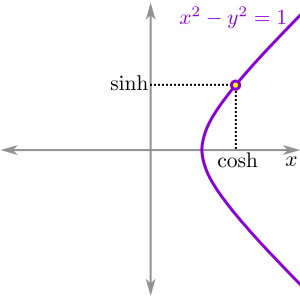
\includegraphics[scale=0.6]{HyperbolicPlot}
\end{center}
\textbf{Example} Using the Taylor series for $e^x$ and substitution, show that the Taylor series for $\cosh$ and $\sinh$ are
\begin{align*}
\cosh(x) &= 1 + \frac{x^2}{2!} + \frac{x^4}{4!} + \dotsb = \sum_{k=0}^\infty \frac{x^{2k}}{(2k)!} \\
\sinh(x) &= x + \frac{x^3}{3!} + \frac{x^5}{5!} + \dotsb = \sum_{k=0}^\infty \frac{x^{2k+1}}{(2k+1)!}. \end{align*}
Note that these are almost the same as the series for cosine and sine, respectively, except they do not alternate. This gives another reason for the names of these functions.\\
Answer:\\
\begin{align*}
\cosh(x) &= \frac{e^x + e^{-x}}{2} \\
&= \frac{1}{2}\left[(1+x+\frac{x^2}{2!} + \dotsb)+(1-x+\frac{x^2}{2!}-\dotsb)\right] \\
&= \frac{1}{2}\left[2 + 2 \frac{x^2}{2!} + 2 \frac{x^4}{4!} +\dotsb \right] \\
&= 1+\frac{x^2}{2!} + \frac{x^4}{4!}+\dotsb \\
&= \sum_{k=0}^\infty \frac{x^{2k}}{(2k)!}.
\end{align*}
\begin{align*}
\sinh(x) &= \frac{e^x - e^{-x}}{2} \\
&= \frac{1}{2}\left[(1+x+\frac{x^2}{2!} + \dotsb)-(1-x+\frac{x^2}{2!}-\dotsb)\right] \\
&= \frac{1}{2}\left[2x + 2 \frac{x^3}{3!} + 2 \frac{x^5}{5!} +\dotsb \right] \\
&= x+\frac{x^3}{3!} + \frac{x^5}{5!}+\dotsb \\
&= \sum_{k=0}^\infty \frac{x^{2k+1}}{(2k+1)!}.
\end{align*}

\subsection{Manipulating Taylor series}
Another way of using one Taylor series to find another is through differentiation and integration. For instance, to find the Taylor series for the derivative of $f$, one can differentiate the Taylor series for $f$ term by term.\\
\textbf{Example} By differentiating the Taylor series for $\sinh$ and $\cosh$, show that
\begin{align*}
\frac{d}{dx} \sinh x &= \cosh x \\
\frac{d}{dx} \cosh x &= \sinh x.
\end{align*}
This is yet another relationship which is similar (though not identical) to the relationship between sine and cosine.\\
Answer:\\
Differentiating hyperbolic sine gives
\begin{align*}
\frac{d}{dx}\sinh x &= \frac{d}{dx}\sum_{k=0}^\infty\frac{x^{2k+1}}{(2k+1)!} \\
&= \sum_{k=0}^\infty (2k+1) \frac{x^{2k}}{(2k+1)!} \\
&= \sum_{k=0}^\infty \frac{x^{2k}}{(2k)!} \\
&= \cosh x,
\end{align*}
as desired. Similarly, differentiating hyperbolic cosine gives
\begin{align*}
\frac{d}{dx}\cosh x &= \frac{d}{dx} \sum_{k=0}^\infty \frac{x^{2k}}{(2k)!} \\
&= \sum_{k=0}^\infty (2k) \frac{x^{2k-1}}{(2k)!} \\
&= \sum_{k=1}^\infty \frac{x^{2k-1}}{(2k-1)!} \\
&= \sum_{k=0}^\infty \frac{x^{2k+1}}{(2k+1)!}.
\end{align*}
There was a little bit of reindexing there, but by writing out a few terms of each series, one can see that all of the above equalities are true.

\subsection{Higher Order Terms in Taylor Series}
In some situations, it will be convenient only to write the first few terms of a Taylor series. This is particularly true when combining or composing more than one Taylor series. Up until now, an ellipsis has been used to indicate that there are more terms in the series that are being omitted.\\
There is another way, sometimes used in this course, of notating the omitted terms in a Taylor series. That is by referring to them as Higher Order Terms (or H.O.T. for short). Having the extra HOT in a series means that all the remaining terms in the series have a higher degree than the previous terms.\\\\
\textbf{Example} The function $e^x$ can be written as \[e^x=1+x+\frac{1}{2!}x^2+\hbox{ HOT},\] or it could also be written as \[e^x=1+x+\hbox{ HOT}.\]
The point at which the higher order terms are cut-off is somewhat arbitrary and depends on the situation. There is a more formal way of keeping track of the higher order terms, called Big-O notation, which is presented in \hyperref[ChFunctionsSecOrdersOfGrowth]{orders of growth}.\\\\
\textbf{Example} Find the first two non-zero terms of the Taylor series for \[f(x)=1-2xe^{\sin x^2}.\]
Answer:\\
Beginning with the innermost function, in this case ${\sin x^2}$, we find that \[\sin x^2=x^2-\frac{1}{3!}(x^2)^3+\hbox{HOT}=x^2-\frac{1}{6}x^6+\hbox{HOT}.\]
Then plugging this into the series for $e^x$ gives
\begin{align*}
e^{\sin x^2}&=1+\left(x^2-\frac{1}{6}x^6+\hbox{HOT}\right)+\frac{1}{2!}\left(x^2+\hbox{HOT}\right)^2+\frac{1}{3!}\left(x^2+\hbox{HOT}\right)^3+\hbox{HOT} \\
&=1+x^2+\frac{1}{2}x^4+\left(-\frac{1}{6}+\frac{1}{6}\right)x^6+\hbox{HOT} \\
&=1+x^2+\frac{1}{2}x^4+\hbox{HOT}
\end{align*}
Then to complete the answer, plug this into the original function to find
\begin{align*}
f(x) &= 1 - 2x \left( 1 + x^2 + \frac{1}{2}x^4 + \hbox{ HOT}\right) \\
&= 1 - 2x - 2x^3 - x^5 + \hbox{ HOT}.
\end{align*}

\subsection{Extra examples}
\textbf{Example}\\
Compute the Taylor series (at 0) for ${\sin^2 x}$ up to and including terms of order 6. Try to give the full Taylor series in summation notation.\\
Answer:\\
\begin{align*}
\sin^2 x &= (x-\frac{x^3}{3!}+\frac{x^5}{5!}-\dotsb)(x-\frac{x^3}{3!}+\frac{x^5}{5!}-\dotsb) \\
&=x^2+(-\frac{1}{3!}-\frac{1}{3!})x^4+(\frac{1}{5!}+\frac{1}{3!\cdot 3!}+\frac{1}{5!})x^6+\dotsb \\
&= x^2-\frac{1}{3}x^4+\frac{2}{45}x^6-\dotsb.
\end{align*}
To get the full Taylor series, one can use the identity \[\sin^2 x=\frac{1-\cos(2x)}{2}\] to find that
\begin{align*}
\sin^2 x &= \frac{1-\cos(2x)}{2} \\
&=\frac{1}{2}\left(1-\left(1-\frac{(2x)^2}{2!}+\frac{(2x)^4}{4!}-\dotsb\right)\right) \\
&=\frac{1}{2}\left(\frac{(2x)^2}{2!}-\frac{(2x)^4}{4!}+\frac{(2x)^6}{6!}-\dotsb\right) \\
&=\frac{1}{2}\sum_{k=1}^\infty(-1)^{k-1}\frac{(2x)^{2k}}{(2k)!}.
\end{align*}
\\\textbf{Example}\\
Find the first three terms of the Taylor series for ${\sqrt{f(x)}}$, where \[f(x)=a_0+a_1 x+a_2 x^2+a_3x^3+\dotsb.\]
Answer:\\
Let ${g(x)=\sqrt{f(x)}}$), where \[g(x)=b_0+b_1 x+b_2 x^2+b_3 x^3+\dotsb.\]
Then ${g(x)^2=f(x)}$, and so the same holds for the Taylor series: \[\left(b_0+b_1 x+b_2 x^2+b_3 x^3+\dotsb\right)^2=a_0+a_1 x+a_2 x^2+\dotsb.\]
Multiplying out and collecting like terms gives \[b_0^2+(b_0b_1+b_1b_0)x+(b_0b_2+b_1b_1+b_2b_0) x^2+\dotsb=a_0+a_1 x+a_2 x^2+\dotsb.\]
Now, equating coefficients of the monomials on the left and right gives the first few equations (of an infinite system of equations)
\begin{align*}
b_0^2 &= a_0 \\ 
2b_0b_1 &= a_1 \\
2b_0b_2 + b_1^2 &= a_2.
\end{align*}
Solving these equations gives the first three coefficients of $g$:
\begin{align*}
b_0 &= \sqrt{a_0} \\
b_1 &= \frac{a_1}{2 \sqrt{a_0}} \\
b_2 &= \frac{1}{2\sqrt{a_0}}\left(a_2-\frac{a_1^2}{4a_0}\right).
\end{align*}
Thus, \[\sqrt{a_0+a_1 x+a_2 x^2+\dotsb}=\sqrt{a_0}+\frac{a_1}{2\sqrt{a_0}}x+\frac{1}{2\sqrt{a_0}}\left(a_2-\frac{a_1^2}{4a_0}\right)x^2+\dotsb.\]

\subsection{Exercises}
\begin{itemize}
\item Compute the Taylor series of ${\cos(2x)\sin(3x)}$ up to and including terms of degree 5. Don't try computing derivatives for this!
\item Use a Taylor polynomial to give a cubic approximation to ${2xe^{3x}}$
\item Compute the Taylor series of ${e^{1-\cos t}}$ in summation notation.
\item Compute the Taylor series of ${\cos(\sin(x))}$ to fourth order.
\item Compute the Taylor series of ${\sin(\cos(x))}$ to forth order. What happens that makes this different than the last problem? (Hint: ${\cos(0)=1}$ but ${\sin(0)=0}$...)
\item Compute the first three nonvanishing terms in the Taylor series of ${e^{2x}(\sinh 3x)/x}$.
\item Compute the Taylor series of ${3x^2 e^{-x^2} \sin 2x^3}$ up to and including terms of order eight! Wow, that means a lot of work, right? Think... which terms should you expand first?
\item Compute the Taylor series of ${\frac{1}{x}e^{-x^2}\sinh(2x)}$ up to the fourth order term.
\item What is the second derivative of the function ${e^{x\cosh(x^2)}}$ at ${x=0}$?
\item Compute the following limit ${\lim_{x\to0}(1-e^x)\frac{\sin(x^2)}{x^3}}$
\end{itemize}

\section{Convergence} \label{ChFunctionsSecConvergence}
A Taylor series can be thought of as an infinite polynomial. Up until now, we have not worried about the issues that come up when adding up infinitely many things. This module deals with two main issues:
\begin{enumerate}
\item A function may not have a Taylor series at all;
\item A function's Taylor series may not converge everywhere, even within the function's domain.
\end{enumerate}
\subsection{Functions without a Taylor series}
The first problem is that some functions cannot be expressed in the form \[ f(x) = \sum_{k=0}^\infty c_k x^k = c_0 + c_1 x + c_2 x^2 + \dotsb \]
Examples include $\tan$, which has vertical asymptotes, and $\ln$, which is not defined for $x \leq 0$. Polynomials are not able to capture these sorts of discontinuities and asymptotes.
\\\textbf{The geometric series}\\
The geometric series is an example of a Taylor series which is well behaved for some values of $x$ and nonsensical for other values of $x$. The claim is that \begin{equation*} 1+x+x^2+x^3+x^4+\dotsb = \frac{1}{1-x}, \end{equation*} for $|x|<1$.
\begin{examplebox}
\textbf{Note} This is not a formal proof, which would require a few tools and definitions we have not yet learned.\\
Let $y = 1+x+x^2+x^3+\dotsb$. Multiplying both sides by $x$ gives
\begin{align*} 
y &= 1 + x + x^2 + x^3 + \dotsb 
x y &= x + x^2 + x^3+x^4 + \dotsb 
\end{align*}
Now, subtracting the second equation from the first, all the terms other than 1 cancel on the right, leaving us with \[ y(1-x) = 1. \]
Dividing by $1-x$ gives $y = \frac{1}{1-x}$.
\end{examplebox}
\textbf{Example} Compute the Taylor series for $f(x) = \frac{1}{1-x}$ directly from the definition.
\begin{examplebox}
\begin{align*} 
f(x) &= \frac{1}{1-x} & f(0) &= 1 \\
f'(x) &= \frac{1}{(1-x)^2} & f'(0) &= 1 \\
f(x) &= \frac{2}{(1-x)^3} & f(0) &= 2 \\
f(x) &= \frac{6}{(1-x)^4} & f(0) &=6. 
\end{align*}	
Notice the pattern that
\begin{equation*} 
f^{\left(k\right)}(x) = \frac{k!}{(1-x)^{k+1}}, 
\end{equation*}	
at least for the first few $k$. To see that the pattern continues, assume it holds for some $k$, and show that it holds for $k+1$ (this is a proof technique known as mathematical induction). If $f^{\left(k\right)}(x) = \frac{k!}{(1-x)^{k+1}}$, then
\begin{equation*}
f^{\left(k+1\right)}(x) = \frac{(k+1)k!}{(1-x)^{k+2}} = \frac{(k+1)!}{(1-x)^{k+2}}, 
\end{equation*}	
as desired. Then $f^{\left(k\right)}(0) = k!$, so according to the definition of Taylor series, it follows that	
\begin{align*} 
\frac{1}{1-x} &= 0! + 1!x+ \frac{2!}{2!}x^2+ \frac{3!}{3!}x^3+\dotsb
&= 1+x+x^2+x^3+\dotsb, 
\end{align*}
which agrees with the above.
\end{examplebox}
\textbf{Note} The geometric series only holds when $|x|<1$. This makes sense, because if $|x|>1$, the powers of $x$ are getting bigger and bigger and so the series should not converge. If $x=1$, then the series is adding 1 infinitely many times, which diverges. If $x=-1$, then the series oscillates between 1 and 0, and hence does not converge.\\
The takeaway is that every Taylor series has a convergence domain where the series is well-behaved, and outside that domain the series will not converge. For many functions, the domain is the whole real number line (e.g. the series for $e^x$, $\sin$, $\cos$, $\cosh$, and $\sinh$ all converge everywhere), but be aware that there are functions whose Taylor series do not converge everywhere. This will be covered more formally in \hyperref[ChSeriesConvergenceAndDivergence]{Series Convergence And Divergence}.\\
\textbf{Example} A beam of light of intensity $L$ hits a pane of glass. Half of the light is reflected, and a third of the light is transmitted; the rest is absorbed. When a beam of light of intensity $L$ hits two parallel panes with an air gap between them, how much light is transmitted through both panes? (The following figure shows how the light gets reflected and rereflected. The first transmitted and reflected beams of light are labeled with their respective intensities. The question asks for the total of the beams of light emerging on the right side of the right pane of glass).
\begin{center}
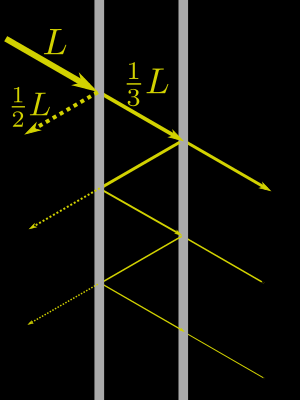
\includegraphics[scale=0.6]{LightGlass}
\end{center}
\begin{examplebox}
By labeling more of the transmitted and reflected beams of light, a pattern emerges among the beams of light on the right side of the right pane:
\begin{center}
	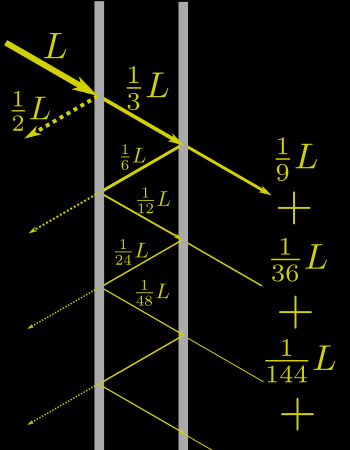
\includegraphics[scale=0.6]{LightGlassSolved}
\end{center}
$\frac{1}{9},\frac{1}{36},\frac{1}{144},\ldots$. Note that each beam is ($\frac{1}{4}$) the previous beam. Thus, the total light emerging on the right side of the right pane of glass is
\begin{align*} 
\frac{L}{9} + \frac{L}{36} + \frac{L}{144}+\dotsb \\
&= \frac{L}{9} \left(1 + \frac{1}{4}+\frac{1}{16}+\dotsb\right) \\
&= \frac{L}{9} \left(\frac{1}{1-1/4}\right) \\
&= \frac{L}{9} \frac{4}{3} \\
&= \frac{4L}{27}, 
\end{align*}
by using the formula for the geometric series.
\end{examplebox}
\textbf{Example} Use the Taylor series of $\frac{1}{1-x}$ to derive the Taylor series of $\ln(1+x)$. Hint: recall that $\ln(1+x) = \int \frac{1}{1+x}dx$.
\begin{examplebox}
Note that
\begin{align*}
\frac{1}{1+x} &= \frac{1}{1-(-x)} \\
&= 1-x+x^2-x^3+x^4-\dotsb.
\end{align*}
Now, integrating gives $\int \frac{dx}{1+x} = \ln(1+x) + C$ on the one hand, and
\begin{align*}
\int (1-x+x^2-x^3+x^4-\dotsb) dx &= x - \frac{x^2}{2} +\frac{x^3}{3} -\dotsb \\
&= \sum_{k=1}^\infty (-1)^{k-1}\frac{x^k}{k}, 
\end{align*}
on the other hand. Plugging in $x=0$ shows that $C=0$, and so
\begin{align*}
\ln(1+x) &= x - \frac{x^2}{2} +\frac{x^3}{3} -\dotsb \\
&= \sum_{k=1}^\infty (-1)^{k+1}\frac{x^k}{k}. \\
& (|x|<1) 
\end{align*}
Note that because this relied on the geometric series, which only holds for $|x|<1$, the same restriction holds for the Taylor series for $\ln(1+x)$.
\end{examplebox}	
\textbf{Example} Use the fact that \[\arctan x = \int \frac{1}{1+x^2}\, dx\] to find the Taylor series for $\arctan x$. 
\begin{examplebox}
Using the fact, and the geometric series, we find that
\begin{align*}
\arctan(x) &= \int \frac{1}{1+x^2} \, dx \\
&= \int \frac{1}{1-\left(-x^2\right)} \, dx \\ 
&= \int \left(1-x^2+x^4-x^6+\dotsb \right) \, dx \\
&= x - \frac{x^3}{3} + \frac{x^5}{5} - \frac{x^7}{7} + \dotsb + C. \\
|x|<1 \\
\end{align*}
Plugging in $x=0$ gives that $C = 0$, since $\arctan 0 = 0$. Thus,
\begin{align*}
\arctan(x) &= x - \frac{x^3}{3}+\frac{x^5}{5}-\dotsb \\
&= \sum_{k=0}^\infty (-1)^k \frac{x^{2k+1}}{2k+1} \\
|x|<1. 
\end{align*}
So even though $\arctan$ is defined for all $x$, its Taylor series only converges for $|x|<1$.
\end{examplebox}
\textbf{Example} Another important function is the binomial series $(1+x)^\alpha$, where $\alpha$ is some constant. Show that
\begin{align*} 
(1+x)^\alpha &= 1 + \alpha x + \frac{\alpha (\alpha - 1)}{2!} x^2 + \frac{\alpha(\alpha-1)(\alpha-2)}{3!} x^3 + \dotsb \\
&= \sum_{k=0}^\infty {\alpha \choose k} x^k, 
\end{align*}
where \[ {\alpha \choose k} = \frac{\alpha (\alpha-1) (\alpha -2) \dotsb (\alpha - k + 1)}{k!}. \] This series also only holds for $|x|<1$.
\begin{examplebox}
For fixed $\alpha$ we have $f(x) = (1+x)^\alpha$. Then proceeding from the definition of the Taylor series, one computes
\begin{align*} 
f(x) &= (1+x)^\alpha & f(0) &= 1 \\
f'(x) &= \alpha(1+x)^{\alpha-1} & f'(0) &= \alpha \\
f(x) &= \alpha(\alpha-1)(1+x)^{\alpha-2} & f(0) &= \alpha(\alpha-1) \\
f(x) &= \alpha(\alpha-1)(\alpha-2)(1+x)^{\alpha-3} & f(0) &= \alpha(\alpha-1)(\alpha-2) \\
& \vdots & \vdots 
\end{align*}
One finds that, in general, $f^{\left(k\right)}(0) = \alpha(\alpha-1)(\alpha-2)\dotsb (\alpha-k+1)$. Thus, the Taylor expansion for $(1+x)^\alpha$ is
\begin{align*}
(1+x)^\alpha &= 1 + \alpha x + \frac{\alpha(\alpha-1)}{2!}x^2 + \frac{\alpha(\alpha-1)(\alpha-2)}{3!}x^3 + \dotsb \\
&= 1 + \binom{\alpha}{1}x + \binom{\alpha}{2}x^2 + \binom{\alpha}{3}x^3 + \dotsb \\
&= \sum_{k=0}^\infty \binom{\alpha}{k} x^k, 
\end{align*}
as claimed.
\end{examplebox}
\subsection{Summary}
Here are all the series we have found so far. The following hold for all $x$:
\begin{align*} 
e^x &= \sum_{k=0}^\infty \frac{x^k}{k!} \\
\cos x &= \sum_{k=0}^\infty (-1)^k \frac{x^{2k}}{(2k)!} \\
\sin x &= \sum_{k=0}^\infty (-1)^k \frac{x^{2k+1}}{(2k+1)!} \\
\cosh x &= \sum_{k=0}^\infty \frac{x^{2k}}{(2k)!} \\
\sinh x &= \sum_{k=0}^\infty \frac{x^{2k+1}}{(2k+1)!}. 
\end{align*}
The following hold for $|x|<1$:
\begin{align*}
\frac{1}{1-x} &= \sum_{k=0}^\infty x^k \\
\ln(1+x) &= \sum_{k=1}^\infty (-1)^{k+1} \frac{x^k}{k} \\
\arctan x &= \sum_{k=0}^\infty (-1)^k \frac{x^{2k+1}}{2k+1} \\
(1+x)^\alpha &= \sum_{k=0}^\infty \binom{\alpha}{k} x^k. 
\end{align*}
\subsection{Electrostatics example}
Here we use the geometric series and the binomial series from above in an example from electrostatics. An electric dipole is a pair of equally and oppositely charged particles separated by a short distance. One question of interest in electrostatics is the electrostatic potential, which is the sum of the point charge potentials from each pole.\\
The point charge potential from a single particle with charge $q$, at a distance $d$ from the particle, is \[ V = \frac{kq}{d}, \] where $k$ is a constant called the Coulomb constant. Then a dipole with particles of charge $q$ and $-q$ has net electrostatic potential \[ V = \frac{kq}{d_+} - \frac{kq}{d_-}, \] where $d_+$ is the distance to the positively charged particle, and $d_-$ is the distance to the negatively charged particle:
\begin{center}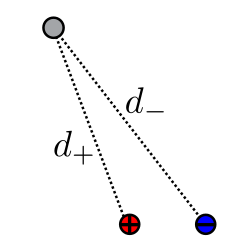
\includegraphics[scale=0.6]{Dipole}\end{center}
We will calculate the first order term for the electrostatic potential at two different locations: $p_1$ and $p_2$:
\begin{center}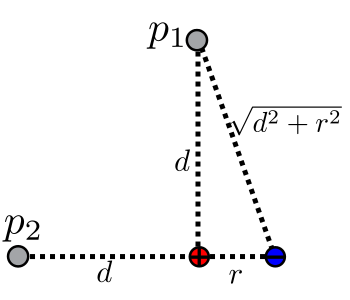
\includegraphics[scale=0.6]{DipolePositions}\end{center}
First consider $p_1$, located directly above and distance $d$ from the positive particle. Let $r$ be the distance between the charged particles. Then $d_+ = d$, and by the Pythagorean theorem, $d_- = \sqrt{d^2+r^2}$. It follows that the electrostatic potential is
\begin{align*} 
V &= \frac{kq}{d_+} - \frac{kq}{d_-} \\
&= \frac{kq}{d} - \frac{kq}{\sqrt{d^2+r^2}}. 
\end{align*}
Now, factoring out $\frac{kq}{d}$, and applying the binomial series with $\alpha = -\frac{1}{2}$, we find
\begin{align*} 
V &= \frac{kq}{d} \left[1 - \frac{1}{\sqrt{1+(r/d)^2}}\right] \\
&= \frac{kq}{d} \left[1 - \left(1+(r/d)^2\right)^{-1/2}\right] \\
&= \frac{kq}{d} \left[1 - \left(1 -\frac{1}{2} (r/d)^2 + \hbox{ HOT}\right)\right] \\
&= \frac{1}{2}\frac{kq r^2}{d^3} + \hbox{ HOT}.
\end{align*}
At position $p_2$, which is directly left of and distance $d$ from the positive particle, we have $d_+ = d$, and $d_- = d+r$, so we find that the electrostatic potential at $p_2$ is
\begin{align*} 
V &= \frac{kq}{d_+} - \frac{kq}{d_-} \\
&= \frac{kq}{d} - \frac{kq}{d+r}. 
\end{align*}
Again, factoring out $\frac{kq}{d}$ and expanding using the geometric series gives
\begin{align*}
V &= \frac{kq}{d} \left(1 - \frac{1}{1+\frac{r}{d}}\right) \\
&= \frac{kq}{d} \left(1 - \left(1 - \frac{r}{d} + \hbox{ HOT}\right)\right) \\
&= \frac{kqr}{d^2} + \hbox{HOT}. 
\end{align*}
\subsection{Exercises}
\begin{itemize}
\item Consider a snowman built from solid snowballs of radius $2^{-n}$, for $n=0,1,2,\ldots $, all stacked on top of one another. How many units tall is the snowman? How many cubic units of snow was required to build it?
\item Compute the Taylor series about zero of \[ \ln\frac{1+3x}{1-3x} \]
\item Compute the Taylor series about zero of \[ \frac{1}{\sqrt{1-x^2}} \]
\item Using your answer to the previous problem, compute the Taylor series about zero of $\arcsin x$, using termwise integration and the fact that \[ \arcsin x = \int \frac{dx}{\sqrt{1-x^2}} \]
\item For which values $z$ is the Taylor series of $\sqrt[4]{3-2z^2}$ guaranteed to converge?
\item Use the binomial series to give the Taylor expansion of $(1+x)^3$. Now, do it with your head: easier, right? Recall, we have said that the binomial series only converges when $|x<1|$, but, clearly, that cannot be a *sharp* constraint, since $(1+x)^3$ is good for all $x$, right? Well, Horatio, there are more things... By the end of this course, we will learn when and how to bend some of these restrictions.
\item Build a cylinder with radius 1 and height 3. Build a second cylinder with radius 1/2 and height 9, a third cylinder with radius 1/4, height 27, a fourth cylinder with radius 1/8 and height 81, and so on. What is the total volume of the cylinders?
\item For which values of $x$ does the Taylor series of $(\frac{1}{4}-3x^2)^{1/4}$ converge?
\end{itemize}

\section{Expansion points} \label{ChFunctionsSecExpansionPoints}
Up until now, Taylor series expansions have all been at $x=0$. The Taylor series at $x=0$ gives a good approximation to the function near 0. But what if we want a good approximation to the function near a different point $a$? That is the topic of this module.
\subsection{Expansion points}
A function $f$ has a Taylor series expansion about any point $x=a$ provided that $f$ and all its derivatives exist at $a$. The definition of the Taylor series for $f$ about $x=a$ is
\begin{align*}
f(x) &= f(a) + f'(a)(x-a) + \frac{f''(a)}{2!}(x-a)^2 + \dotsb \\
&= \sum_{k=0}^\infty \frac{f^{\left(k\right)}(a)}{k!}(x-a)^k. 
\end{align*}
We say this is a series in $(x-a)$. A different way to view this series is by making the change of variables $x = a+h$. After cancellation, this yields
\begin{align*} 
f(a+h) &= f(a) + f'(a)h + \frac{f''(a)}{2!}h^2 + \dotsb \\
&= \sum_{k=0}^\infty \frac{f^{\left(k\right)}(a)}{k!}h^k. 
\end{align*}
\subsection{Taylor polynomial for approximation}
Recall that the first few terms of the Taylor series for $f$ about $x=0$ gives a polynomial (the Taylor polynomial) which is a good approximation for $f$ near 0. Similarly, the Taylor polynomial for $f$ about $x=a$ gives a polynomial which is a good approximation of $f$ near $x=a$. Note, however, that as the input gets further away from the expansion point $a$, the approximation gets worse.
\textbf{Example} Find the Taylor series for $f(x) = 3x^2-x+4$ about $x=2$.
\begin{examplebox}
Computing the derivatives, and evaluating at ($x=2$), one finds
\begin{align*}
f(x) &= 3x^2-x+4 & f(2) &= 14 \\
f'(x) &= 6x-1 & f'(2) &= 11 \\
f(x) &= 6 & f(2) &= 6 \\
f(x) &= 0 & f(2) &= 0. 
\end{align*}
And all the subsequent derivatives are 0. So from the definition, one finds that
\begin{align*}
f(x) &= 14 + 11(x-2) + \frac{6}{2!}(x-2)^2 \\
&= 14 + 11(x-2) + 3(x-2)^2.
\end{align*}
This appears to be different than the polynomial $f$ with which we began. If one multiplies out this polynomial and collects like terms, however, the result is the original polynomial. This should not be surprising, since the best polynomial approximation to a polynomial is the polynomial itself, even factored into a slightly different form.
\end{examplebox}
\textbf{Example} Compute the Taylor series expansion for $\ln(x)$ about $x=1$. 
\begin{examplebox}
Begin by computing the first few derivatives and evaluating at $x=1$:
\begin{align*}
f(x) &= \ln(x) & f(1) &= 0 \\
f'(x) &= x^{-1} & f'(1) &=1 \\
f(x) &= -x^{-2} & f(1) &= -1 \\
f(x) &= 2x^{-3} & f(1) &= 2.
\end{align*}
The pattern that emerges is $f^{\left(k\right)}(x) = (-1)^{k-1}(k-1)!x^{-k}$. To see that the pattern holds, check that
\begin{equation*}
f^{\left(k+1\right)}(x) = (-1)^{k-1} (-k)(k-1)!x^{-k-1} = (-1)^k k! x^{-(k+1)},
\end{equation*}
as desired. So by induction, the pattern holds. It follows that $f^{\left(k\right)}(1) = (-1)^{k-1}(k-1)!$ for $k \geq 1$. Plugging in to the formula, one finds that
\begin{align*} 
\ln(x) &= \sum_{k=1}^\infty \frac{(-1)^{k-1}(k-1)!}{k!}(x-1)^k \\
&= \sum_{k=1}^\infty (-1)^{k-1} \frac{(x-1)^k}{k} \\
&= (x-1) - \frac{(x-1)^2}{2} + \frac{(x-1)^3}{3} - \frac{(x-1)^4}{4}+\dotsb.
\end{align*}
Note that with the change of variables $h = x-1$ (and hence $x = h+1$, we find that \[ \ln(1+h) = h - \frac{h^2}{2} + \frac{h^3}{3} - \frac{h^4}{4} + \dotsb, \] which is the same series we found earlier for  $\ln(1+x)$.
\end{examplebox}
Note that the Taylor polynomial is only a good approximation to the function on the domain of convergence. For functions whose domain of convergence is the entire number line, this is not a concern. But for functions such as $\ln x$, the Taylor polynomials will only be a good approximation within the domain of convergence, which is $0 < x < 2$. Outside of that domain, the Taylor polynomials diverge wildly from $\ln x$, as shown here:
\begin{center}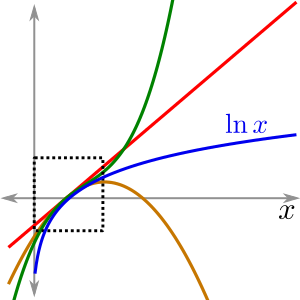
\includegraphics[scale=0.6]{NaturalLogApproximation}\end{center}
Even within a function's domain of convergence, a Taylor polynomial's approximation gets worse as the input gets further away from $a$. One way to improve an approximation is to include more and more terms of the Taylor series in the Taylor polynomial. However, this involves computing more and more derivatives. Another way to improve the approximation for $f(x)$ is to choose an expansion point $a$ which is close to $x$.\\
\textbf{Example} Use the Taylor polynomial of degree 2 for $f(x) = \sqrt{x}$ about $x=1$ to approximate $\sqrt{10}$. Then repeat the process about $x=9$ and compare the results. 
\begin{examplebox}
Using the definition, one finds
\begin{align*}
f(x) &= \sqrt{x} & f(1) &= 1 & f(9) &= 3 \\
f'(x) &= \frac{1}{2\sqrt{x}} & f'(1) &= \frac{1}{2} & f'(9) &= \frac{1}{6} \\
f(x) &= -\frac{1}{4x^{3/2}} & f(1) &= -\frac{1}{4} & f''(9) &= -\frac{1}{108} 
\end{align*}
Thus, the Taylor polynomial about $x=1$ is
\begin{align*}
\sqrt{x} & \approx 1 + \frac{1}{2}(x-1) - \frac{1/4}{2!}(x-1)^2 \\
&= 1 + \frac{1}{2}(x-1) - \frac{1}{8}(x-1)^2.
\end{align*}
And the corresponding approximation is
\begin{align*} 
\sqrt{10} &\approx 1 + \frac{1}{2}\cdot 9 - \frac{1}{8} \cdot 9^2 \\
&\approx -4.6, 
\end{align*}
which is obviously quite far off the mark. On the other hand, the Taylor polynomial about $x=9$ is
\begin{align*}
\sqrt{x} & \approx 3 + \frac{1}{6}(x-9) - \frac{1/{108}}{2!}(x-9)^2 \\
&= 3 + \frac{1}{6}(x-9) - \frac{1}{216}(x-9)^2.
\end{align*}
And the corresponding approximation is
\begin{align*}
\sqrt{10} &\approx 3 + \frac{1}{6}\cdot 1 - \frac{1}{216} \cdot 1^2 \\
&\approx 3.1620, 
\end{align*}
which is quite a good approximation of $\sqrt{10}\approx 3.1623$.
\end{examplebox}
\subsection{Caveat for compositions}
When computing the Taylor expansion for the composition $f \circ g$ about $x=a$, one must be careful of expansion points. In particular, one cannot simply take the series for $g$ at $x=a$ and plug it into the series for $f$ at $x=a$.\\
\textbf{Example} Consider the expansion for $e^{\cos(x)}$ about $x=0$. Although $\cos(x) = 1-\frac{x^2}{2!} +\dotsb$, and $e^x = 1+x+\frac{x^2}{2!}+\dotsb$, one will run into trouble trying to write
\begin{equation*}
e^{\cos(x)} = 1+(1-\frac{x^2}{2!} +\dotsb) + \frac{1}{2}(1-\frac{x^2}{2!} +\dotsb)^2 + \dotsb.
\end{equation*}
The trouble is that collecting like terms requires adding up infinitely many things. For instance, the constant term above is $1+1+\frac{1}{2}+\dotsb$. The reason this is a problem is that Taylor series are supposed to give a good polynomial approximation of a function without requiring too much computation or information about the function.\\
Remember that $e^x = 1+x+\frac{x^2}{2}+\dotsb$ is a good approximation when $x$ is near 0. However, when $x$ is near 0, $\cos(x)$ is near 1. So plugging the series for $\cos(x)$ into the series for $e^x$ does not give a good approximation. \\
To avoid this problem when computing the Taylor series for the composition $f \circ g$ at $x=a$, one should plug the Taylor expansion of $g$ about $x=a$ into the expansion of $f$ about $x=g(a)$. In the above example, the expansion of $e^x$ about $x=1$ is
\begin{equation*}
e^x = e + e(x-1) + \frac{e}{2!}(x-1)^2 + \dotsb,
\end{equation*}
so
\begin{align*}
e^{\cos(x)} &= e + e\left[\left(1-\frac{x^2}{2!}+\dotsb\right)-1\right] + \frac{e}{2!}\left[\left(1-\frac{x^2}{2!}+\dotsb\right)-1\right]^2 + \dotsb \\
&= e + e(-\frac{x^2}{2} + \dotsb) + \frac{e}{2}(-\frac{x^2}{2}+\dotsb)^2 + \dotsb \\
&= e - \frac{e}{2}x^2 + \dotsb.
\end{align*}
\subsection{Exercises}
\begin{itemize}
\item Without using a calculator, find a decimal approximation to $\sqrt{83}$ by Taylor-expanding $\sqrt{x}$ about $a=81$ and using the zero-th and first order terms.
\item Without using a calculator, find a decimal approximation to $\sqrt[3]{124}$ using linear approximation. How close was your answer to truth?	
\item Without using a calculator, find a decimal approximation to $\cos(1)$ [in radians!] using linear approximation. How close was your answer to truth? (Hint: $\pi/3\approx 1$...)
\item Taylor expand $\sin x$ about $x=\pi$ and compute all the terms. Does what you get make sense?
\item Use completing the square and the geometric series to get the Taylor expansion about $x=2$ of $\frac{1}{x^2+4x+3}$
\item Approximate $1004^{1/3}$ using the zeroth and first order terms of the Taylor series.
\end{itemize}

\section{Limits} \label{ChFunctionsSecLimits}

Having concluded our study of Taylor series, we now move on to limits. Some of the major topics of calculus (continuity, differentiation, and integration) can all be expressed using limits.

\subsection{Definition of the limit}
The limit formalizes the behavior of a function as its input approaches some value. The formal definition of the limit is
\begin{examplebox}
Limit $\displaystyle \lim_{x \rightarrow a} f(x) = L$ if and only if for every $\epsilon>0$ there exists $\delta>0$ such that $|f(x)-L|<\epsilon$ whenever $0<|x-a|<\delta$. If there is no such $L$, then the limit does not exist.
\end{examplebox}
In words, this says that the limit of a function exists if, when the input to $f$ is very close to $a$ (but not equal to $a$), the output from $f$ is very close to $L$. This can also be thought of in terms of tolerances: given a certain $\epsilon$ tolerance for the output (seen as the band around $L$ in the graph below), one can find a tolerance $\delta$ on the input (the band around $a$) so that for inputs within the tolerance, the corresponding outputs stays within $\epsilon$ of the desired output:
\begin{center}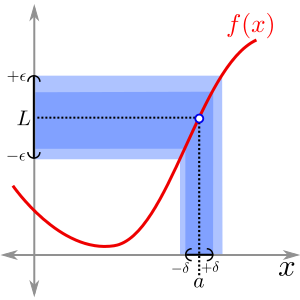
\includegraphics[scale=0.6]{Limit}\end{center}

No matter how small $\epsilon$ is made, there must be some $\delta$, which must depend on $\epsilon$, generally. Actually finding $\delta$ often requires a little bit of work.

\textbf{Example} Using the definition of the limit, show that $\displaystyle \lim_{x \rightarrow 3} x^2 = 9$. 
\begin{examplebox}
\textbf{Note} This is rather technical, and is only a demonstration of the process required to prove a limit exists from the definition. This course deals almost exclusively with continuous functions, where such proofs are not necessary.

We must show that for any given $\epsilon>0$, there exists $\delta$ (which depends on $\epsilon$) such that $0<|x-3|<\delta$ implies $|x^2-9|<\epsilon$.
Let $\epsilon>0$ be given. A little bit of algebra shows that \[ |x^2-9| = |x-3| \cdot |x+3|. \]
We get to control $|x-3|$ with $\delta$. We also have (by using the triangle inequality) that \[ |x+3| = |x-3+6| \leq |x-3|+6 < \delta + 6. \]
Thus, \[ |x^2-9| = |x-3|\cdot |x+3| < \delta \cdot (\delta + 6). \]
Now, if we pick $\delta$ to be the minimum of $1$ and $\frac{\epsilon}{7}$, then we simultaneously guarantee that $\delta \leq \frac{\epsilon}{7}$ and $\delta + 6 \leq 7$, and so we find \[ |x^2-9| < \delta \cdot (\delta + 6) \leq \frac{\epsilon}{7} \cdot 7 = \epsilon, \] as desired.
\end{examplebox}
\subsection{When limits may not exist}
There are a few ways a limit might not exist:
\begin{enumerate}
	\item A \textit{discontinuity}, or jump, in the graph of the function. In this case, the limit does not exist because the limit from the left and the limit from the right are not equal.
	\item A \textit{blow-up}, when the function has a vertical asymptote.
	\item An \textit{oscillation}, where the graph of the function oscillates infinitely up and down as the input approaches a certain value.
\end{enumerate}
\begin{center}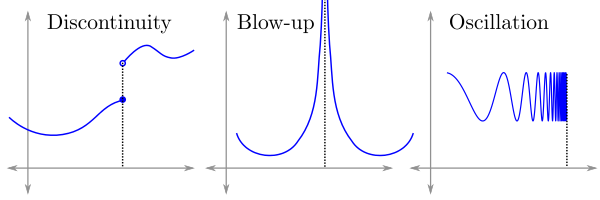
\includegraphics[scale=0.6]{LimitFails}\end{center}
Most functions in this course will be well-behaved and will not have the above problems. The formal term for a well-behaved function is continuous.

\subsection{Continuous functions}
A function is continuous at the point ($a$) if the limit ($\lim_{x \rightarrow a} f(x)$) exists and ($\lim_{x \rightarrow a} f(x) = f(a)$). Intuitively, this says that there are no holes or jumps in the graph of ($f$) at ($a$).\\
Finally, a function is continuous if it is continuous at every point in its domain.

\subsection{Rules for limits}
There are rules for adding, multiplying, dividing, and composing limits. Suppose that $\displaystyle \lim_{x \rightarrow a} f(x)$ and $\displaystyle \lim_{x \rightarrow a} g(x)$ exist. Then
\begin{enumerate}
\item (Sum) $\displaystyle \lim_{x \rightarrow a} (f+g)(x) = \lim_{x \rightarrow a} f(x) + \lim_{x \rightarrow a} g(x)$.
\item (Product) $\displaystyle \lim_{x \rightarrow a} (f \cdot g)(x) = \left(\lim_{x \rightarrow a}f(x)\right)\left(\lim_{x \rightarrow a} g(x)\right)$.
\item (Quotient) $\displaystyle \lim_{x \rightarrow a} \left(\frac{f}{g}\right)(x) = \frac{\lim_{x \rightarrow a} f(x)}{\lim_{x \rightarrow a} g(x)}$, provided that $\displaystyle \lim_{x \rightarrow a} g(x) \neq 0$.
\item (Chain) $\displaystyle \lim_{x \rightarrow a} (f \circ g)(x) = f\left(\lim_{x \rightarrow a} g(x)\right)$, if $f$ is continuous.
\end{enumerate}

Almost all the functions encountered in this course are continuous, and so limits in most cases can be evaluated by simply plugging in the limiting input value into the function. The one case that sometimes gets complicated is the Quotient rule above when the limit of the denominator is 0.

\textbf{Example} Show that $\displaystyle \lim_{x\rightarrow 0}\frac{\sin(x)}{x} = 1$. 
\begin{examplebox}
There are several proofs of this limit (e.g. memorization, l'Hospital's rule), but the simplest method is to use the Taylor series. Because $x$ is near 0, the Taylor series expansion for $\sin x$ applies, and so
\begin{align*}
\lim_{x \rightarrow 0} \frac{\sin(x)}{x} &= \lim_{x\rightarrow 0} \frac{x-\frac{x^3}{3!}+\dotsb}{x} \\
&= \lim_{x\rightarrow 0} \frac{x \left(1-\frac{x^2}{3!}+\dotsb\right)}{x} \\
&= \lim_{x\rightarrow 0} 1-\frac{x^2}{3!} +\dotsb \\
&= 1. 
\end{align*}
This works because all the terms involving $x$ go to 0 as $x$ goes to 0.
\end{examplebox}

\textbf{Example} Find $\displaystyle \lim_{x\rightarrow 0} \frac{1-\cos x}{x}$. 
\begin{examplebox}
Replacing $\cos$ with its Taylor series (again, since $x$ is near 0), we find
\begin{align*} 
\lim_{x \rightarrow 0} \frac{1-\cos x}{x} &= \lim_{x \rightarrow 0} \frac{1-\left(1-\frac{1}{2!}x^2 + \frac{1}{4!}x^4 - \dotsb \right)}{x} \\
&= \lim_{x \rightarrow 0} \frac{\frac{1}{2!}x^2 - \frac{1}{4!}x^4 + \dotsb}{x} \\
&= \lim_{x \rightarrow 0} \frac{1}{2!}x - \frac{1}{4!}x^3 + \dotsb \\
&= 0. 
\end{align*}
\end{examplebox}

\textbf{Example} Compute $\displaystyle \lim_{x\rightarrow 0} \frac{\cos(x)-\sin(x)-1}{e^x-1}$. 
\begin{examplebox}
Again, use the Taylor series about $x=0$ for each function: 
\begin{align*}
\lim_{x \rightarrow 0} \frac{\cos(x)-\sin(x)-1}{e^x-1} &= \lim_{x \rightarrow 0} \frac{(1-\frac{x^2}{2!}+\dotsb)-(x-\frac{x^3}{3!}+\dotsb)-1}{(1+x+\frac{x^2}{2!}+\dotsb)-1} \\
&= \lim_{x\rightarrow 0}\frac{-x-\frac{x^2}{2!}+\dotsb}{x+\dotsb} \\
&= \lim_{x \rightarrow 0} \frac{x(-1-\dotsb)}{x(1+\dotsb)} \\
&= \lim_{x \rightarrow 0} \frac{-1-\dotsb}{1+\dotsb} \\
&= -1.
\end{align*}
\end{examplebox}

\textbf{Example} Compute $\displaystyle \lim_{x \rightarrow 0} \frac{\sqrt[3]{1+4x} - 1}{\sqrt[5]{1+3x} - 1}$.
\begin{examplebox}
Here, we use the binomial series with $\alpha = \frac{1}{3}$ in the numerator, and $\alpha = \frac{1}{5}$ in the denominator. We find
\begin{align*}
\lim_{x \rightarrow 0} \frac{(1+4x)^{1/3}- 1}{(1+3x)^{1/5} - 1} &= \lim_{x \rightarrow 0} \frac{\left(1+\frac{1}{3}(4x) + \hbox{ HOT}\right)-1}{\left(1+\frac{1}{5}(3x) + \hbox{ HOT}\right) - 1} \\
&= \lim_{x \rightarrow 0} \frac{\frac{4}{3}x + \hbox{ HOT}}{\frac{3}{5}x + \hbox{ HOT}} \\
&= \lim_{x \rightarrow 0} \frac{\frac{4}{3} + \hbox{ HOT}}{\frac{3}{5} + \hbox{ HOT}} \\
&= \frac{\frac{4}{3}}{\frac{3}{5}} \\
& = \frac{20}{9}
\end{align*}
\end{examplebox}
There are other methods for computing these types of limits, including memorization, algebraic tricks, and l'Hopital's rule (more on that in the next module). However, in many cases, these different methods can all be replaced by a simple application of Taylor series.

\section{Exercises}
Compute the following limits:
\[ \displaystyle \lim_{q \to 1} \frac{q^2 + q + 1}{q+3} \]
\[ \displaystyle \lim_{x \to -2} \frac {x^2-4}{x+2} \]
\[ \displaystyle \lim_{x \to 0} \frac{\sec x\tan x}{\sin x} \]
\[ \displaystyle \lim_{x \to +\infty} \frac{6x^2 -3x+1}{3x^2+4} \]
\[ \displaystyle \lim_{x \rightarrow +\infty} \frac {x^2+x+1}{x^4-3x^2+2} \]
\[ \displaystyle \lim_{y \to 0} \frac{\ln(1+2y)\sin y}{y^2\cos 2y} \]
\[ \displaystyle \lim_{x\to 1} \frac{\ln x}{x^2} \]
\[ \displaystyle \lim_{t\to 0} (3t^2+4t)\cot(t) \]
\[ \displaystyle \lim_{z\to 0} \frac{z\cos(\sin(z))}{\sin(2z)} \]
\[ \displaystyle \lim_{x \to 0} \frac{\ln (x+1)\arctan x}{x^2} \]
\[ \displaystyle \lim_{x \to 0} \frac{\ln^2(\cos x)}{2x^4-x^5} \]
\[ \displaystyle \lim_{s \to 0} \frac{e^s s \sin s}{1 - \cos 2s} \]
\[ \displaystyle \lim_{x \to 0^+} \frac{\sin(\arctan(\sin x))}{\sqrt{x} \sin 3x +x^2+ \arctan 5x} \]
\[ \displaystyle \lim_{x \to 0} \frac{\sin x -\cos x -1}{6x e^{2x}} \]
\[ \displaystyle \lim_{x \to 0} \frac{\arctan x-3 \sin x +2x}{3x^3} \]
\[ \displaystyle \lim_{p \to 0} \frac{1-p- \cos 3p}{p^3} \]
\[ \displaystyle \lim_{x \to \infty} x^{1/x} \]

\section{L'Hopital's Rule} \label{ChFunctionsSecLHopitalsRule}
In previous modules, we saw that Taylor series are useful for computing certain limits of ratios. But sometimes, a fact known as L'Hopital's rule is easier to use than Taylor series. While L'Hopital's rule is commonly taught in a first calculus course, the justification for why it works is not usually taught. This module gives a justification for L'Hopital's rule, using Taylor series.

\subsection{L'Hopital's rule}
There are some limit situations where Taylor series are not particularly easy to use. For example, if the limit is being taken at a point about which the Taylor expansion is not already known, or the limit is at infinity, then using Taylor series is usually more work than it is worth. These are the situations where L'Hopital's rule can be helpful.
\begin{definitionbox}[title=\textbf{L'Hopital's Rule, $\frac{0}{0}$ case}]
If $f$ and $g$ are continuous functions such that $\displaystyle \lim_{x \rightarrow a} f(x) = 0$ and $\displaystyle\lim_{x \rightarrow a} g(x) = 0$, then $\displaystyle \lim_{x \rightarrow a} \frac{f(x)}{g(x)} = \lim_{x\rightarrow a} \frac{f'(x)}{g'(x)}$, provided this limit exists. If this is still of the form $\frac{0}{0}$, then derivatives may be taken again, and so on.
\end{definitionbox}

\begin{examplebox}
The Taylor series for $f$ and $g$ about $a$ are given by
\begin{align*}
f(x) &= f(a) + f'(a)(x-a) + \frac{f(a)}{2!}(x-a)^2+ \dotsb \\
g(x) &= g(a) + g'(a)(x-a) + \frac{g(a)}{2!}(x-a)^2 + \dotsb. 
\end{align*}
Since, by hypothesis, $f(a) = g(a) = 0$, it follows that
\begin{align*}
\lim_{x\rightarrow a} \frac{f(x)}{g(x)} &= \lim_{x \rightarrow a} \frac{ f(a) + f'(a)(x-a) + \frac{1}{2}f(a)(x-a)^2 + \dotsb}{g(a) + g'(a)(x-a) + \frac{1}{2}g(a)(x-a)^2+\dotsb} \\
&= \lim_{x\rightarrow a} \frac{f'(a) (x-a) +(1/2)f(a)(x-a)^2 + \dotsb}{g'(a)(x-a) + (1/2)g(a)(x-a)^2+ \dotsb} \\
&= \lim_{x \rightarrow a} \frac{(x-a)\left[f'(a) + (1/2)f(a)(x-a) + \dotsb \right]}{(x-a)\left[g'(a) + (1/2)g(a)(x-a) + \dotsb \right]} \\
&= \lim_{x \rightarrow a} \frac{f'(a) + (1/2)f(a)(x-a) + \dotsb }{g'(a) + (1/2) g(a)(x-a) + \dotsb}.
\end{align*}
Now, as $x \rightarrow a$, all the terms with $x-a$ go to 0, which leaves $\frac{f'(a)}{g'(a)}$. If this fraction is still $0/0$, then L'Hopital's rule says to take the derivative of the numerator and the denominator again. In terms of the Taylor series, this moves to the next leading terms in the numerator and denominator.
\end{examplebox}

\textbf{Example} Using L'Hopital's rule, compute two of the limits from the last module:
\begin{align*}
\lim_{x \rightarrow 0} & \frac{\sin x}{x} \\
\lim_{x \rightarrow 0} & \frac{1-\cos x}{x}. 
\end{align*}
\begin{examplebox}
These are both in the ($\frac{0}{0}$) case, so differentiating numerator and denominator gives
\begin{align*}
\lim_{x \rightarrow 0} \frac{\sin x}{x} &= \lim_{x \rightarrow 0} \frac{\cos x}{1} \\
&= 1. 
\end{align*}
\begin{align*}
\lim_{x \rightarrow 0} \frac{1-\cos x}{x} &= \lim_{x \rightarrow 0} \frac{\sin x}{1} \\
&= 0.
\end{align*}
\end{examplebox}

\textbf{Example} Compute $\displaystyle \lim_{x \rightarrow 0} \frac{\tan x}{\arcsin x}$.
\begin{examplebox}
Since $\tan 0 = \arcsin 0 = 0$, we are in the $\frac{0}{0}$ case of L'Hopital's rule. Recall that
\begin{align*}
\frac{d}{dx} \tan x &= \sec^2 x \\
\frac{d}{dx} \arcsin x &= \frac{1}{\sqrt{1-x^2}}.
\end{align*}
Thus, applying L'Hopital's rule gives
\begin{align*}
\lim_{x \rightarrow 0} \frac{\tan x}{\arcsin x} &= \lim_{x \rightarrow 0} \frac{ \sec^2 x }{ \frac{1}{\sqrt{1-x^2}} } \\
&= \frac{1}{1} \\
&= 1.
\end{align*}
\end{examplebox}
Depending on the situation, it still might be easier to use Taylor series, especially if there are compositions and products of functions (assuming we know all the relevant Taylor series).

\textbf{Example} Compute $\displaystyle \lim_{x \rightarrow 0} \frac{x^2 \ln( \cos x)}{\sin^2(3x^2)} $. 
\begin{examplebox}
We know all the relevant Taylor series for the functions in this problem, so that should be an easier method. We find
\begin{align*}
\lim_{x\rightarrow 0} \frac{x^2 \ln(\cos x)}{\sin^2(3x^2)} &= \lim_{x \rightarrow 0} \frac{x^2 \ln \left(1-\frac{x^2}{2!} + \hbox{ HOT}\right)}{\left(3x^2 + \hbox{ HOT}\right)^2} \\
&= \lim_{x \rightarrow 0} \frac{x^2 \left(-\frac{x^2}{2} - \hbox{ HOT}\right)}{9x^4 + \hbox{ HOT}} \\
&= \lim_{x \rightarrow 0} \frac{-\frac{x^4}{2} + \hbox{ HOT}}{9 x^4 + \hbox{ HOT}} \\
&= -\frac{1}{18}. 
\end{align*}
Using L'Hopital here would be quite a lot of work. It turns out that we would have to apply the rule four times, which involves a lot of product and chain rule.
\end{examplebox}

\begin{definitionbox}[title=\textbf{L'Hopital's Rule, $\frac{\infty}{\infty}$ case}]
If $\displaystyle \lim_{x\rightarrow a} f(x) = \lim_{x \rightarrow a} g(x) = \infty$, then $\displaystyle\lim_{x \rightarrow a} \frac{f(x)}{g(x)} = \lim_{x\rightarrow a} \frac{f'(x)}{g'(x)}$, again provided this limit exists.	
\end{definitionbox}

\textbf{Example} Compute $\displaystyle \lim_{x \rightarrow 0} \frac{\ln x}{\frac{1}{x^2}}$.
\begin{examplebox}
Note that $\ln x \rightarrow -\infty$ as $x \rightarrow 0$, and $\frac{1}{x^2} \rightarrow \infty$ as $x \rightarrow 0$. Therefore, the $\frac{\infty}{\infty}$ case of L'Hopital's rule applies. Applying the rule,
\begin{align*}
\lim_{x \rightarrow 0} \frac{\ln x}{x^{-2}} &= \lim_{x \rightarrow 0} \frac{\frac{1}{x}}{-2 x^{-3}} \\
&= \lim_{x\rightarrow 0} \frac{x^2}{-2} \\
&= 0.
\end{align*}
\end{examplebox}

\textbf{Example} Use L'Hopital's rule to compute $\displaystyle \lim_{x\rightarrow \pi} \frac{\sin(x)}{e^x \cos(x/2)}$. 
\begin{examplebox}
Since $\sin, \cos, \exp$ are all continuous functions, and $\sin(\pi) = e^{\pi} \cos (\pi/2) = 0$, the hypotheses for L'Hopital's rule are met. So it follows that
\begin{align*}
\lim_{x\rightarrow \pi} \frac{\sin(x)}{e^x \cos(x/2)} &= \lim_{x\rightarrow \pi} \frac{[\sin(x)]'}{[e^x \cos(x/2)]'} \\
&= \lim_{x \rightarrow \pi} \frac{\cos(x)}{e^x \cos(x/2) -(1/2)e^x\sin(x/2)} \\
&= \frac{-1}{0 - (1/2)e^{\pi} \sin(\pi/2)} \\
&= 2e^{-\pi}. 
\end{align*}
Note that although we know the Taylor series for these functions at $x=0$, the limit here is as $x \rightarrow \pi$. Thus, we cannot use the Taylor series approach, because a Taylor series about $x=0$ does not give a good approximation when $x$ is not close to 0.
\end{examplebox}

\subsection{Other indeterminate forms}
Some limits do not initially look like cases where L'Hopital's rule applies, but with some algebra they can be rearranged into one of the applicable cases. These are called indeterminate forms.\\\\
\textbf{Case: $\infty - \infty$}\\

First, consider $\displaystyle \lim_{x \rightarrow a} f(x) - g(x)$, where $\displaystyle \lim_{x \rightarrow a} f(x) = \lim_{x\rightarrow a} g(x) = \infty$. Usually, one or both of $f$ and $g$ are ratios of other functions. In this case, getting a common denominator usually transforms the limit into one where L'Hospital's rule or a Taylor series approach applies.

\textbf{Example} Compute $\displaystyle \lim_{x \rightarrow 0} \frac{1}{\sin^2 x} - \frac{1}{x^2}$. 
\begin{examplebox}
Getting a common denominator, and then Taylor expanding gives
\begin{align*}
\lim_{x \rightarrow 0} \frac{1}{\sin^2x} - \frac{1}{x^2} &= \lim_{x\rightarrow 0} \frac{x^2 - \sin^2x}{x^2 \sin^2x } \\
&= \lim_{ x\rightarrow 0} \frac{x^2 - \left(x-\frac{1}{3!}x^3 + \dotsb \right)^2}{x^2 \left(x- \frac{1}{3!}x^3 + \dotsb\right)^2} \\
&= \lim_{x \rightarrow 0} \frac{x^2 - \left(x^2 - \frac{2}{3!}x^4 + \dotsb\right)}{x^2 \left(x^2 - \frac{2}{3!}x^3 + \dotsb\right)} \\
&= \lim_{x \rightarrow 0} \frac{\frac{2}{6}x^4 + \dotsb}{x^4 + \dotsb} \\
&= \frac{1}{3}.
\end{align*}
\end{examplebox}
\bigbreak
\noindent \textbf{Case: $\infty \cdot 0$}\\

Next, consider $\displaystyle \lim_{x \rightarrow a} f(x)g(x)$ where $\displaystyle \lim_{x \rightarrow a} f(x) = \infty$ and $\displaystyle \lim_{x \rightarrow a}g(x) = 0$. Since $\infty \cdot 0$ is not defined, it is not clear what this limit is. However, the product can be turned into one of the following ratios where L'Hopital's rule applies:
\begin{align*}
\lim_{x \rightarrow a} f(x)g(x) &= \lim_{x \rightarrow a} \frac{g(x)}{1/f(x)} \\
&= \lim_{x \rightarrow a} \frac{f(x)}{1/g(x)}
\end{align*}
since dividing by the reciprocal of a number is the same as multiplying. Now, note that $\displaystyle \lim_{x \rightarrow a} 1/f(x) = 0$, since $\displaystyle \lim_{x \rightarrow a} f(x) = \infty$. Thus, $ \displaystyle \lim_{x \rightarrow a} \frac{g(x)}{1/f(x)}$ is now in the $\frac{0}{0}$ case of L'Hopital's rule.

Similarly, $\displaystyle \lim_{x \rightarrow a} \frac{f(x)}{1/g(x)}$ is in the $\frac{\infty}{\infty}$ form of l'Hopital's rule, and so it can be applied here too.

Deciding which of the above forms to use depends on the situation, but in many situations either form will work.

\textbf{Example} Compute $\displaystyle \lim_{x \rightarrow 0^+} x \ln x$. (Here we use the one-sided limit $x \rightarrow 0^+$ becuase $\ln$ is only defined on the positive real numbers).
\begin{examplebox}
This is of the form $0 \cdot (-\infty)$. In this case, it is easier to flip $x$ into the denominator, because it is easier to take the derivative of $x^{-1}$ than it is to take the derivative of $(\ln x)^{-1}$. So, we find
\begin{align*}
\lim_{x \rightarrow 0^+} x \ln x &= \lim_{x \rightarrow 0^+} \frac{ \ln x}{x^{-1}},
\end{align*}
which is of the form $\frac{-\infty}{\infty}$, so applying L'Hopital's rule gives
\begin{align*}
\lim_{x \rightarrow 0^+} \frac{ \ln x}{x^{-1}} &= \lim_{x \rightarrow 0^+} \frac{x^{-1}}{-x^{-2}} \\
&= \lim_{x \rightarrow 0^+} -x \\
&= 0.
\end{align*} 
\end{examplebox}
\bigbreak
\noindent \textbf{Case: $\infty^0$}\\

Another indeterminate form arises when raising one function of $x$ to a power which involves another function of $x$. Suppose $\displaystyle \lim_{x \rightarrow a} f(x) = \infty$ and $\displaystyle \lim_{x \rightarrow a} g(x) = 0$. Then what is $\displaystyle \lim_{x \rightarrow a} f(x)^{g\left(x\right)}$?

On the one hand, it seems that raising $\infty$ to any power should be $\infty$. On the other hand, raising anything to the 0th power should be 1. To find what the answer actually is, let \[ y = \lim_{x \rightarrow a} f(x)^{g\left(x\right)}, \] and take the $\ln$ of both sides. Now, recall that $\ln$ is a continuous function. Therefore, from the rules of limits in the last module, taking $\ln$ of a limit is the same as the limit of the $\ln$:
\begin{align*}
\ln(y) &= \ln\left(\lim_{x\rightarrow a} f(x)^{g\left(x\right)}\right) \\
&= \lim_{x \rightarrow a} \ln \left(f(x)^{g\left(x\right)}\right) \\
&= \lim_{x \rightarrow a} g(x) \ln(f(x))
\end{align*}
(the last step uses the fact that $\ln(a^b) = b\ln(a)$). Now, this is of the form $0 \cdot \infty$, which was covered above. Note that when this limit is computed, it is $\ln(y)$ which has been found, and so the answer must be exponentiated to find $y$, the original limit.

\textbf{Example} Compute $\displaystyle \lim_{x \rightarrow \infty} x^{1/x}$. 
\begin{examplebox}
This is of the $\infty^0$ form. Let $\displaystyle y = \lim_{x \rightarrow \infty} x^{1/x}$. Then taking $\ln$ gives
\begin{align*}
\ln(y) &= \lim_{x \rightarrow \infty} \ln\left(x^{1/x}\right) \\
&= \lim_{x \rightarrow \infty} \frac{1}{x}\ln(x) \\
&= \lim_{x \rightarrow \infty} \frac{\ln x}{x} \\
&= \lim_{x \rightarrow \infty} \frac{1/x}{1} \\
&= 0 
\end{align*}
(L'Hopital's rule was used in the second to last step).\\
So $\ln(y) = 0$, and so $y = 1$ is the answer.
\end{examplebox}

\section{Orders of growth} \label{ChFunctionsSecOrdersOfGrowth}

\chapter{Differentiation} \label{ChDifferentiation}
\section{Derivatives} \label{ChDifferentiationSecDerivatives}
\section{Differentiation rules} \label{ChDifferentiationSecDifferentiationRules}
\section{Linearization} \label{ChDifferentiationSecLinearization}
\section{Higher derivatives} \label{ChDifferentiationSecHigherDerivatives}
\section{Optimization} \label{ChDifferentiationSecOptimization}
\section{Differentials} \label{ChDifferentiationSecDifferentials}
\section{Differentiation as an operator} \label{ChDifferentiationSecDifferentiationAsAnOperator}

\chapter{Integration} \label{ChIntegration}
\section{Antidifferentiation} \label{ChIntegrationSecAntidifferentiation}
\section{Exponential growth examples} \label{ChIntegrationSecExponentialGrowthExamples}
\section{More differential equations} \label{ChIntegrationSecMoreDifferentialEquations}
\section{ODE Linearization} \label{ChIntegrationSecODELinearization}
\section{Integration by Substitution} \label{ChIntegrationSecIntegrationBySubstitution}
\section{Integration by parts} \label{ChIntegrationSecIntegrationByParts}
\section{Trigonometric substitution} \label{ChIntegrationSecTrigonometricSubstitution}
\section{Partial fractions} \label{ChIntegrationSecPartialFractions}
\section{Definite integrals} \label{ChIntegrationSecDefiniteIntegrals}
\section{Fundamental Theorem of Integral Calculus} \label{ChIntegrationSecFundamentalTheoremOfIntegralCalculus}
\section{Improper integrals} \label{ChIntegrationSecImproperIntegrals}
\section{Trigonometric integrals} \label{ChIntegrationSecTrigonometricIntegrals}
\section{Tables and computers} \label{ChIntegrationSecTablesAndComputers}

\chapter{Applications} \label{ChApplications}

\chapter{Discretization} \label{ChDiscretization}
\section{Series} \label{ChDiscretizationSecSeries}

\end{sloppypar}
\end{document}
